% Paper template for Advanced Physics Laboratory Course
% Suggestion: it is better to compile it directly on overleaf, because the subfigure settings can arise problems
% Made by Alice Pagano and Francesca Dodici

\documentclass[rmp,10pt,onecolumn,fleqn,notitlepage]{revtex4-1}

% LOAD PACKAGES

% GENERAL PACKAGES
\usepackage{graphicx}
\usepackage{wrapfig}
\usepackage{color}
\usepackage{latexsym,amsmath}
\usepackage{physics}
\usepackage{chemformula}
\usepackage{tabularx}
\usepackage{float}
\usepackage{siunitx}
\usepackage{amssymb}
\usepackage{amsmath}
\usepackage{listings}
\usepackage[caption=false]{subfig} % rovina la formattazione delle figure se caption=true

\usepackage[qm]{qcircuit} % Quantum circuit

\usepackage{multirow}

% LISTING PACKAGES
\usepackage{xcolor}
\usepackage{listings}
\usepackage{framed}
\usepackage{inconsolata} % To change the listing font

% URL PACKAGE AND SETTING
\definecolor{linkcolor}{rgb}{0,0,0.65} %hyperlink
\definecolor{linescolor}{rgb}{0.65,0.16,0.16}
\definecolor{cool}{RGB}{49,54,149}
\definecolor{hot}{RGB}{165,0,38}
\usepackage[pdftex,colorlinks=true, pdfstartview=FitV, linkcolor= linescolor, citecolor= linescolor, urlcolor= linkcolor, hyperindex=true,hyperfigures=true]{hyperref} %hyperlink%


% LISTING SETTINGS
\definecolor{codegray}{rgb}{0.5,0.5,0.5}
\definecolor{commentcolour}{rgb}{0.43,0.63,0.65}
\definecolor{darkgreen}{rgb}{0.0, 0.5, 0.0}

\lstdefinestyle{myPython}{
    language=Python,
    backgroundcolor=\color{white},
    commentstyle=\color{commentcolour},
    keywordstyle=\bfseries\color{darkgreen},
    numberstyle=\tiny\color{codegray},
    stringstyle=\color{hot},
    basicstyle=\ttfamily\footnotesize,
    breakatwhitespace=false,
    breaklines=true,
    captionpos=b,
    keepspaces=true,
    arc=5mm,
    %numbers=left,
    %numbersep=5pt,
    showspaces=false,
    showstringspaces=false,
    showtabs=false,
    tabsize=2
    %frame=single,
    %framexleftmargin=11pt
}


% PAGE SETTING
\usepackage{fancyhdr}

\pagestyle{fancyplain}
\fancyhf{}
\fancyfoot[R]{\textbf{\thepage}}
\fancyfoot[L]{Quantum Information and Computing (a.y. 2020/21) - Diparimento di Fisica e Astronomia Galileo Galilei}
%\fancyhead[L]{\textbf{Advanced Physics Laboratory Report}}
\fancyhead[L]{\ifnum\value{section}>0\nouppercase{\textbf{\leftmark}\fi}}
\fancyhead[R]{\textbf{A. Pagano - M. Puppin}}
\renewcommand{\headrulewidth}{0.2pt}
\renewcommand{\footrulewidth}{0.1pt}

\setlength\parindent{9pt} % To adjust the intendation

% SECTION STYLE
%Redefine \thesubsection as \thesection.\alph{subsection}. (\alph replaces the default \arabic; you could also choose, e.g., \Alph, \roman, and \Roman.)
\renewcommand{\thesection}{\textbf{\Roman{section}}}
\renewcommand{\thesubsection}{\textbf{\arabic{subsection}}}
\renewcommand{\thesubsubsection}{\textbf{\Alph{subsubsection}}}
%\renewcommand{\thesection}{\textbf{\arabic{section}}}
%\renewcommand{\thesubsection}{\thesection.\textbf{\arabic{subsection}}}
%\renewcommand{\thesubsubsection}{\textbf{\thesection.\arabic{subsection}.\arabic{subsubsection}}}

\makeatletter
\renewcommand{\paragraph}{% standard vertical spacing: 3.25ex
    \@startsection{paragraph}{4}%
    {\z@}{2.50ex \@plus 1ex \@minus .2ex}{-1em}%
    {\bf\sffamily}%
}
\makeatother

% FIGURE AND TABLE STYLE
\renewcommand{\tablename}{\textbf{TAB.}}
\renewcommand{\thetable}{\textbf{\arabic{table}}}

% Eliminare nella compilazione finale
\renewcommand{\figurename}{\textbf{FIG.}}
\renewcommand{\thefigure}{\textbf{\arabic{figure}}}

% BIBLIOGRAPHY FILE AND SETTING
\bibliographystyle{aipnum4-1}
\setcitestyle{numbers,square}



\begin{document}


% FRONTESPIZIO

% Insert logo images above
\begin{figure}[H]
\begin{minipage}{0.25\linewidth}

\includegraphics[width=\linewidth]{image/logo/logo_DFA.jpg}
\end{minipage}
\hfill
\begin{minipage}{0.35\linewidth}

\includegraphics[width=\textwidth]{image/logo/logo_800anni.png}
\end{minipage}
\end{figure}

% Make upper lines
\noindent\makebox[\linewidth]{\color{linescolor} \rule{0.85\paperwidth}{1.2 pt}}
\noindent\makebox[\linewidth]{\color{linescolor} \rule[0.3cm]{0.85\paperwidth}{1pt}}

% Title
\title{Two-qubit CZ gate implementation with trapped neutral atoms: \\ a numerical simulation}
\author{
    \parbox{3.0cm}{Alice Pagano}       \parbox{2.5cm}{Mat. 1236916} \parbox{6.0cm}{\bf\href{mailto:alice.pagano@studenti.unipd.it}{\texttt{alice.pagano@studenti.unipd.it}}}          \\
    \parbox{3.0cm}{Michele Puppin} \parbox{2.5cm}{Mat. 1227474} \parbox{6.0cm}{\bf\href{mailto:michele.puppin@studenti.unipd.it}{\texttt{michele.puppin@studenti.unipd.it}}}}
%\author{Alice Pagano - 1236916 - alice.pagano@studenti.unipd.it \\ Michele Puppin - 1227474 - michele.puppin@studenti.unipd.it}
\date{\today}

% Abstract
\begin{abstract}

Multi-qubit gates can be implemented with trapped neutral atoms by driving them to highly excited Rydberg states, in which nearby Rydberg atoms can interact very strongly and in a controlled way. In this Report, we simulate the dynamics of a system under the application of a controlled-phase gate physically implemented in \cite{PhysRevLett.123.170503}. After a physical and theoretical description of the two-qubit CZ gate design, the dynamics of a two-qubit system is simulated in both the perfect and imperfect Rydberg blockade regime by varying the optimal parameters suggested. Then, we consider the CZ gate in the case of a chain of $N$-qubit. A Gaussian noise is introduced on the optimal parameters to investigate noise effects with an increasing number of qubits.
Numerical methods for performing unitary time evolution are also discussed and their performances are tested.



\end{abstract}

% Make title
\maketitle

% Make lower line
\noindent\makebox[\linewidth]{\color{linescolor} \rule[0.1cm]{0.85\paperwidth}{1pt}}


% INDEX

% Index configuration
{
  \hypersetup{linkcolor=black}
  \tableofcontents
}
% Make lower lines
\noindent\makebox[\linewidth]{\color{linescolor} \rule[-0.2cm]{0.85\paperwidth}{1pt}}
\noindent\makebox[\linewidth]{\color{linescolor} \rule[0.3cm]{0.85\paperwidth}{1.2 pt}}
\pagebreak


% Page configuration: start counting page after the first one which is the title
\pagenumbering{gobble}
\newpage
\pagenumbering{arabic}






\section{Introduction}
\label{sec:introduction}

Nowadays, many research groups and companies are investing time and resources for the development of practical quantum computers.
The basic idea of a quantum computer is much the same of a classical one. The information is stored in a register of \textit{qubits}, namely quantum mechanical systems with two orthogonal states conventionally denoted by $\ket{0}$ and $\ket{1}$.
The processing tasks are carried out by \textit{quantum logic gates}. These quantum logic gates are connected together in a \textit{quantum circuit} in order to carry out specified processing tasks \cite{10.5555/1200964}.
It has not yet been decided which basic physical principle is the most suitable for physical implementations of qubits and in general the most important functional parameters of a quantum computer. According to current knowledge, the most promising physical systems for building a next-generation quantum computer are superconductors, atomic traps and ion traps.

In recent years, quantum operations with \textit{trapped neutral atoms} have made significant progress and have reached values in the range of those of ion traps and superconductors.
Indeed, single atom initialization, addressing and readout have been demonstrated in a variety of optical trapping platforms and single-qubit gates have been implemented with exquisite fidelity \cite{PhysRevLett.123.170503}.
Moreover, multi-qubit gates can be implemented with neutral atoms by driving them to highly excited \textit{Rydberg states}.
These are states with large principal quantum numbers $n$.
Consequently, an atom in this state has a diameter which is approximately a factor of $10^4$ larger than that of a neutral atom in the ground state. However, it is not an ion, as this outer electron is not free, but is still bound, even if very weakly.
It is therefore very sensitive to external electromagnetic influences and, consequently, the nearby Rydberg atoms interact very strongly and in a controlled way. This allows for example the realization of conditional quantum logic gates.

In this project, a physical implementation \cite{PhysRevLett.123.170503} of a two-qubit CZ gate (up to a global gauge choice) between individual neutral atoms trapped in optical tweezer is numerically simulated. More specifically, a CZ gate is an example of a \textit{controlled unitary operator gate}. It has two input qubits, which are designated as the \textit{control} and \textit{target} qubits, respectively. The gate has no effect on the control qubit, but performs a unitary operation on the target qubit conditionally on the state of the control qubit \cite{Fox:1001868}. For instance, for a two-qubit CZ gate the $Z$ operator is applied to the target qubit conditional upon the state of the control qubit, resulting in a matrix representation as in Eq. \eqref{eq:controlled-Zgate}.

\begin{equation}
\begin{minipage}[c]{0.3\linewidth}
    $CZ = 
    \begin{pmatrix}
     1 & 0 & 0 & 0 \\ 
     0 & 1 & 0 & 0 \\ 
     0 & 0 & 1 & 0 \\
     0 & 0 & 0 & -1
    \end{pmatrix}$
\end{minipage}
\begin{minipage}[c]{0.2\linewidth}
    \Qcircuit @C=1em @R=2em {
    & \qw &\ctrl{1} & \qw & \qw \\
    & \qw & \gate{Z}  & \qw & \qw
    }  
\end{minipage}
\label{eq:controlled-Zgate}
\end{equation}

First of all, we discuss the physical and theoretical design of the two-qubit CZ gate. Optimal values for the pulse duration $\tau$, the detuning $\Delta$ and the Rabi frequency $\Omega$ are needed to reproduce exactly its behavior.

Then, we describe in details the numerical simulation of the two-qubit CZ gate both in the case of perfect and imperfect blockade regime. We make use of QuTip, a Python library which provides  ready-use  functions to  handle  quantum  systems. After that, the CZ gate is generalized to a chain of $N$-qubit.
In both the two-qubit and chain of $N$-qubit system, a Gaussian noise is introduced and noise effects are investigated. 

Since for a $N$-qubit system the dimension of the total Hamiltonian scales as $3^N\times3^N$, the time evolution of the system can become computationally challenging for larger $N$. Hence, methods to perform unitary time evolution in an optimal way are discussed and coded with different implementations. 
A timing analysis is performed in order to compare different methods and implementations. 

All the implemented code and the results shown in this work are available on GitHub \cite{github}.



\clearpage

\section{Physical implementation of single-qubit and two-qubit gates}
\label{sec:physical_implementation}
% Fisica e diretto riferimento alla costruzione matemetica che porta alla Hamiltoniana

In the real experiment conducted by H. Levine et All. \cite{PhysRevLett.123.170503}, individual neutral atoms are trapped in \textit{optical tweezers} and organized in a one-dimensional array into groups of two. Qubits are encoded in hyperfine ground states of these atoms with $\ket{0}=\ket{5 S_{1/2}, F=1, m_F=0 }$ and $\ket{1}=\ket{5 S_{1/2}, F=2, m_F=0 }$. 


\begin{figure}[H]
    \fontsize{10pt}{12pt}\selectfont
    \begin{minipage}{0.5\linewidth}\setlength{\parindent}{9pt}
    \paragraph{Optical pumping into $\pmb{\ket{0}}$.} First of all, all qubits are initialized in $\ket{0}$ through a Raman-assisted optical pumping procedure as illustrated in Fig. \ref{fig:raman-optical-pumping}. Atoms into all $m_F$ states within the $\ket{5 S_{1/2}, F=1}$ manifold are coarse pumped and a Raman $\pi$-pulse is applied to excite from $\ket{F=1,m_F=-1}$ to $\ket{F=2,m_F=-1}$ and from $\ket{F=1,m_F=+1}$ to $\ket{F=2,m_F=+1}$. Then, the system is coarse pumped back from $F=2$ to $F=1$. The effect is that some population from $\ket{F=1,m_F=\pm 1}$ is transferred to $\ket{F=1,m_F=0}$. The cycle is repeated $N \sim 70$ times to achieve a net population of $99.3\%$ in $\ket{0}$.
    More specifically, the transition between qubit states $\ket{0}$ and $\ket{1}$ is driven by a 795 nm Raman laser aligned along the array of atoms. It is $\sigma^+$ polarized to coherently drive $\pi$ transitions between $F=1$ and $F=2$ ground state manifolds with a Rabi frequency of $\Omega_{01}= 2 \pi \times \SI{250}{kHz}$. 
    \end{minipage}
    \hfill
    \begin{minipage}{0.45\linewidth}
    \centering
     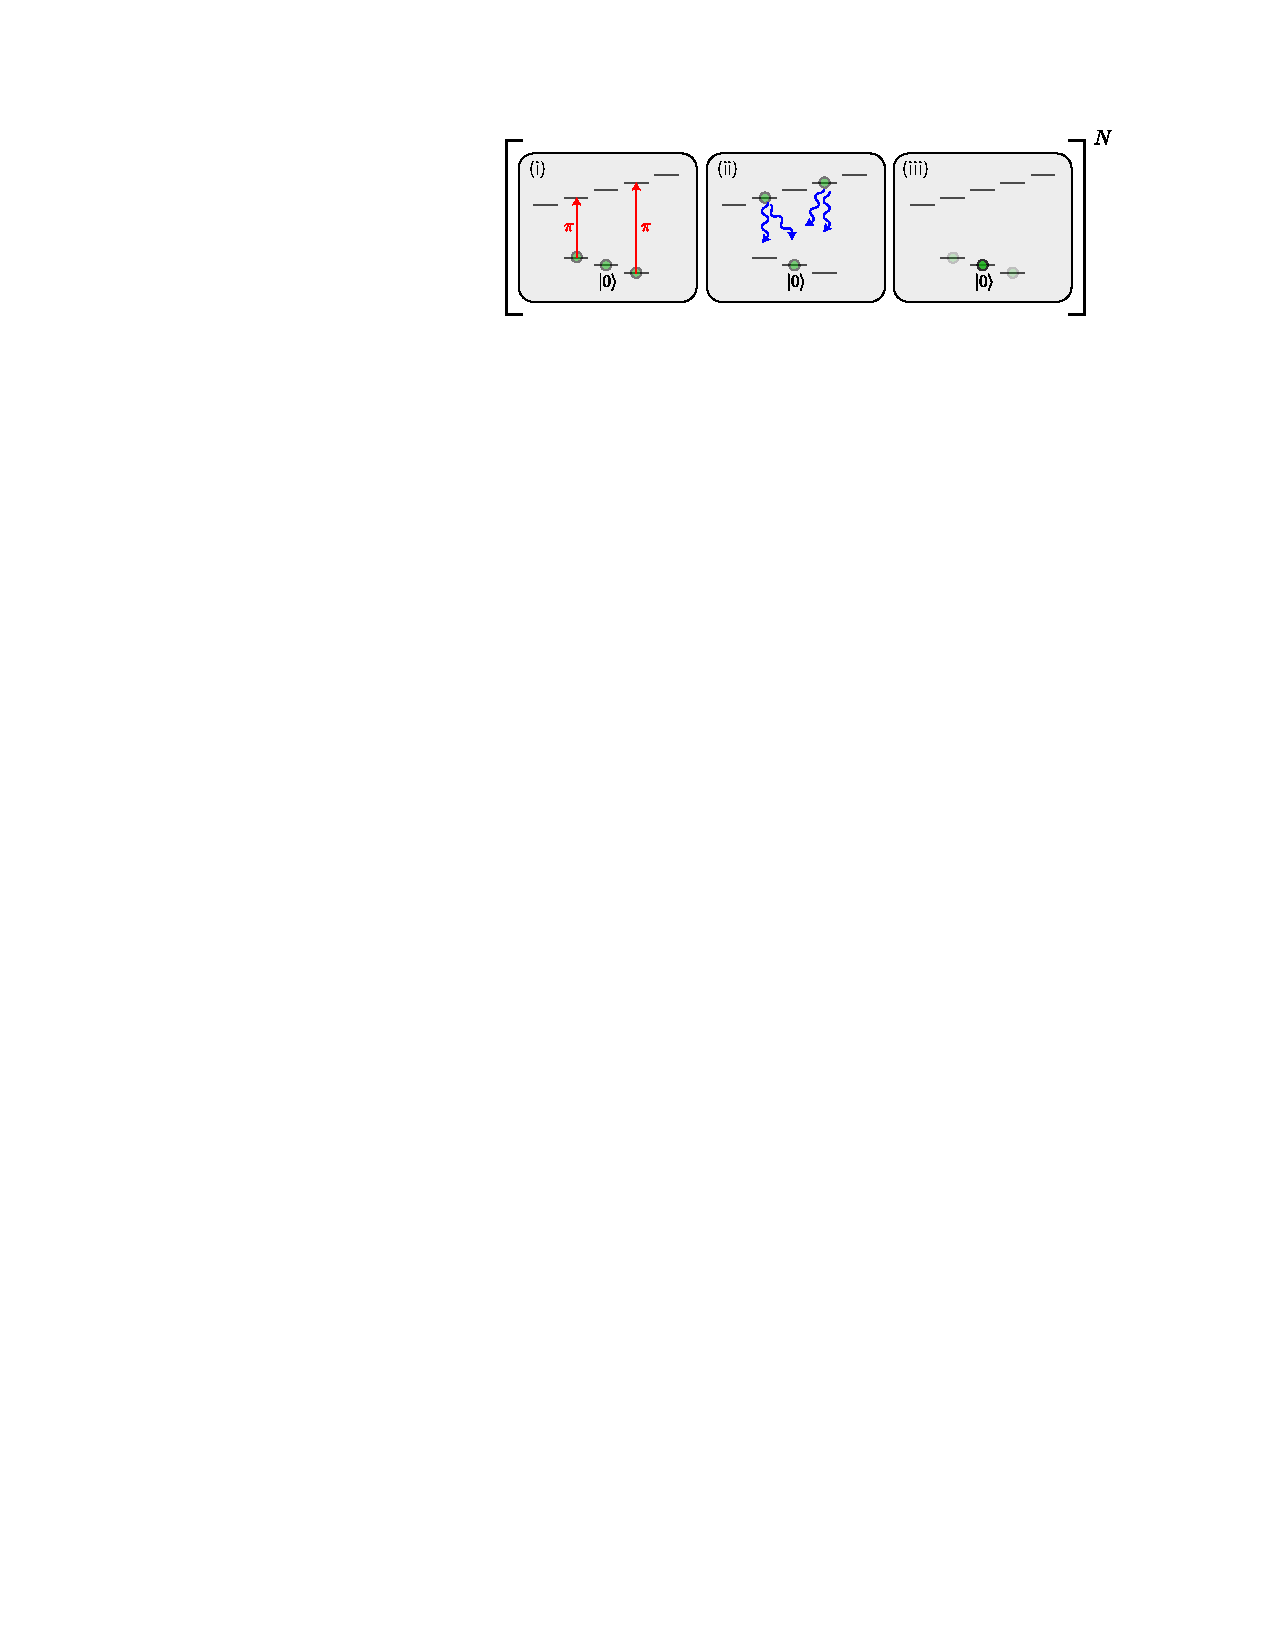
\includegraphics[width=1\textwidth]{image/physical_implementation/raman-optical-pumping.pdf}
    \caption{ Raman-assisted optical pumping scheme (repeated $N$ times) \cite{PhysRevLett.123.170503}. \textbf{(i)} All three sublevels of $F=1$ are coarse pumped and a Raman $\pi$-pulse is applied to excite from $\ket{F=1,m_F=-1}$ to $\ket{F=2,m_F=-1}$ and from $\ket{F=1,m_F=+1}$ to $\ket{F=2,m_F=+1}$. \textbf{(ii)} The system is coarse pumped back from $F=2$ to $F=1$. \textbf{(iii)} Some population from $\ket{F=1,m_F=\pm 1}$ is transferred to $\ket{F=1,m_F=0}$.  }
    \label{fig:raman-optical-pumping}
    \end{minipage}
\end{figure}

\paragraph{Single-qubit gates.} Single-qubit gates are implemented through a combination of the global 795 nm laser beam which homogeneously and simultaneously drives all qubits in the one-dimensional array and of local 420 nm beams focused onto individual sites, resulting in a light shift $\delta$ used for individual addressing (Fig. \ref{fig:one-dimensional-array}). These two coupling are described by $X(\theta)$ global qubit rotation and $Z(\theta)$ local rotations. More specifically, the two single-qubit gates physically implemented in the experiment are $X(\pi/4)$ and $Z(\pi)$.
	
	\begin{figure}[h!]
	    \centering
	    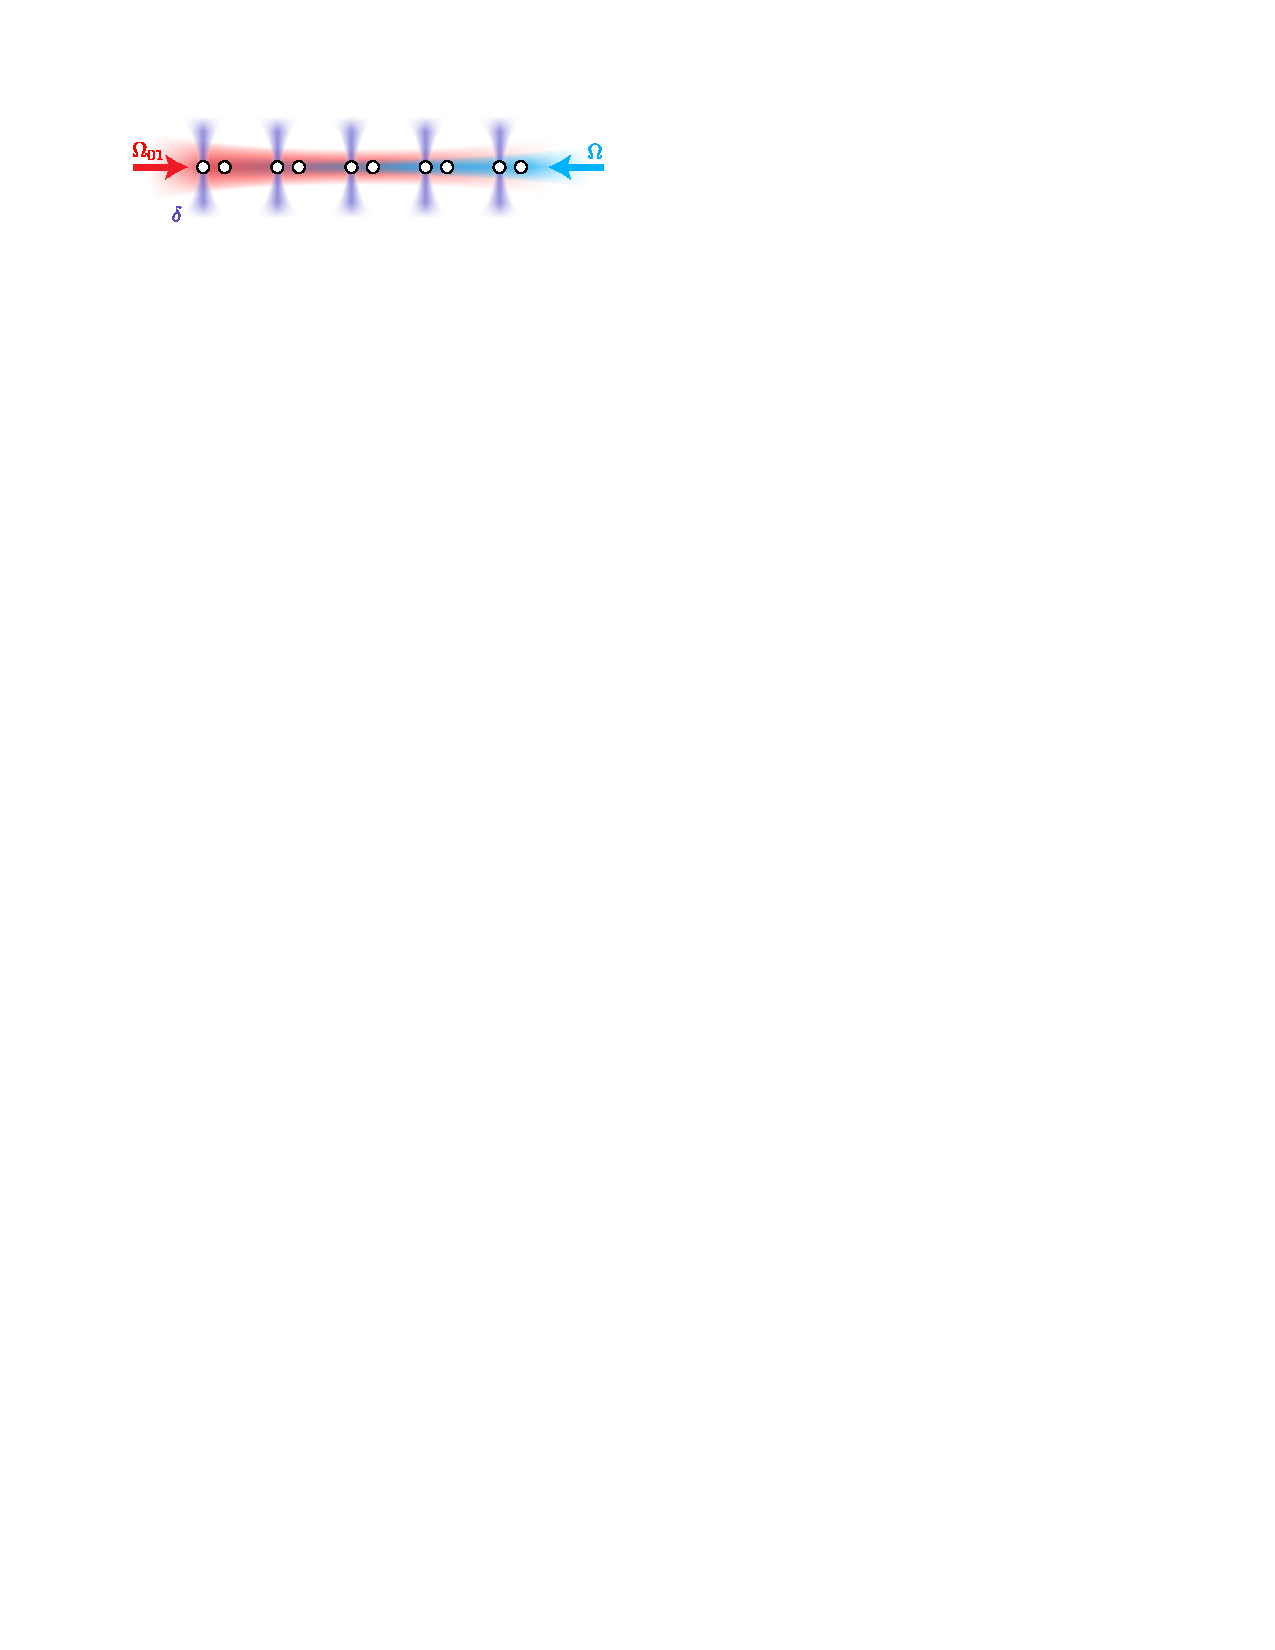
\includegraphics[width=0.5\textwidth]{image/physical_implementation/one-dimensional-array.pdf}
	    \caption{One-dimensional array of neutral atoms \cite{PhysRevLett.123.170503}. Atoms are arranged in pairs and are globally driven with a 795 nm Raman laser (in red) which couples the qubit states $\ket{0}$ and $\ket{1}$. Local 420 nm (purple) beams are focused onto individual atoms. Atoms are globally excited by a bi-chromatic, 420 nm and 1013 nm, Rydberg laser (blue) from the $\ket{1}$ qubit state to $\ket{r}$. }
	    \label{fig:one-dimensional-array}
	\end{figure}

For a two qubits system, both initialized in $\key{0}$, all the four computational basis states are experimentally initialized using global $X(\pi/2)$ pulses (two sequential $X(\pi/4)$ gates) and local $Z(\pi)$ gates on the left atom only (top qubit in each circuit):

\begin{itemize}
    \item the $\ket{00}$ requires no pulses to prepare;
    \item the $\ket{01}$ state is prepared as follows:
          \begin{equation*}
            \Qcircuit @C=0.8em @R=1.1em {
            \lstick{\ket{0}} & \qw	& \gate{X(\pi/2)} & \gate{Z(\pi)}	 & \gate{X(\pi/2)}  & \qw  & \qw & \stick{\ket{0}} \\  
            \lstick{\ket{0}} & \qw	& \gate{X(\pi/2)} & \qw	 & \gate{X(\pi/2)}  & \qw & \qw & \stick{\ket{1}} \\  
            }
          \end{equation*}
    \item the $\ket{10}$ state is prepared as follows:
          \begin{equation*}
            \Qcircuit @C=0.8em @R=1.1em {
            \lstick{\ket{0}} & \qw	& \gate{X(\pi/2)} & \gate{Z(\pi)}	 & \gate{X(3 \pi/2)}  & \qw  & \qw & \stick{\ket{1}} \\ 
            \lstick{\ket{0}} & \qw	& \gate{X(\pi/2)} & \qw	 & \gate{X(3\pi/2)}  & \qw & \qw & \stick{\ket{0}} \\  
            }
          \end{equation*}
    \item the $\ket{11}$ state requires only a global $X(\pi)$ gate.
\end{itemize}

 
\paragraph{Two-qubit gates.} Two-qubit gates are physically implemented by exciting atoms from the qubit state $\ket{1}$ to the Rydberg state $\ket{r}=\ket{70 S_{1/2}, m_J=-1/2 }$ trough a two-photon process with effective Rabi frequency $\Omega \approx 2 \pi \times \SI{3.5}{\MHz}$. The coupling from $\ket{1}$ to $\ket{r}$ is obtained through a bi-chromatic laser system. In particular, the laser at 420 nm is polarized to drive a $\sigma^-$ transition through the intermediate state $\ket{6 P_{3/2}}$, while the one at 1013 nm to drive a $\sigma^+$ transition. The relevant atomic levels for realizing two-qubit gates are summarized in Fig. \ref{fig:atomic-levels}.

	\begin{figure}[h!]
	    \centering
	   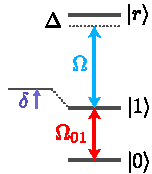
\includegraphics[width=0.2\textwidth]{image/physical_implementation/atomic-levels.pdf}
	    \caption{Relevant atomic levels \cite{PhysRevLett.123.170503}.  The qubit states $\ket{0}=\ket{5 S_{1/2}, F=1, m_F=0}$ and $\ket{1}=\ket{5 S_{1/2}, F=2, m_F=0}$ are coupled with Rabi frequency $\Omega_{01}$. $\delta$ is the light shift used for individual addressing resulting from local 420 nm beams.
	    The qubit state $\ket{1}$ is coupled to the Rydberg state $\ket{r}=\ket{70 S_{1/2}, m_J=-1/2}$ with detuning $\Delta$ and effective Rydberg Rabi frequency $\Omega$.}
	    \label{fig:atomic-levels}
	\end{figure}
	
A new protocol for implementing a two-qubit \textbf{controlled-phase} (\textbf{CZ}) \textbf{gate} consists of just two global laser pulses (with the laser phase of the second pulse shifted by $\xi$) of the same length $\tau$ and detuning $\Delta$ which couple $\ket{1}$ to $\ket{r}$ and drive nearby atoms within the Rydberg blockade regime. Indeed, within a given cluster of atoms the strength of the Rydberg interaction is strong, i.e. $2 \pi \times \SI{24}{\MHz} \gg \Omega$, since atoms are trapped  sufficiently close to each other. Therefore, neighboring atoms cannot be simultaneously excited to the Rydberg state according to the \textit{Rydberg blockade}. The desired CZ gate (up to global rotation of qubits) maps the computational basis states as follows:
\begin{equation}
    \begin{aligned}
        \ket{00} & \rightarrow \ket{00} \\
        \ket{01} & \rightarrow \ket{01} e^{i\phi} \\
        \ket{10} & \rightarrow \ket{10} e^{i\phi}\\
        \ket{11} & \rightarrow \ket{11} e^{i(2\phi-\pi)}\\
    \end{aligned}
    \label{eq:CZ-gate-map}
\end{equation}
The behavior of the four computational basis states is: 
\begin{itemize}
    \item the $\ket{00}$ state does not evolve since it is uncoupled by the laser field;
    \item the dynamics of $\ket{01}$ (and $\ket{10}$) are given by the coupling of the single atom on the $\ket{1} \leftrightarrow \ket{r}$ transition forming a two-level system with Rabi frequency $\Omega$ and detuning $\Delta$ (Fig. \ref{fig:01-dynamics});
    \item the $\ket{11}$ state evolves within the Rydberg blockade regime as a two-level system due to the collective coupling from $\ket{11} \leftrightarrow \ket{W} = \frac{1}{\sqrt{2}}(\ket{1r}+\ket{r1})$, with enhanced Rabi frequency $\sqrt{2}\Omega$ and the same detuning $\Delta$ (Fig. \ref{fig:11-dynamics}).
\end{itemize}

    \begin{figure}[h!]
    \begin{minipage}[c]{0.49\linewidth}
    \centering
    \subfloat[][Dynamics of $\ket{01}$ state. ]{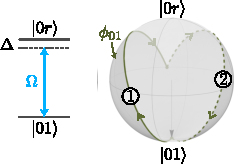
\includegraphics[width=0.4\textwidth]{image/physical_implementation/01-dynamics.pdf} \label{fig:01-dynamics} }
    \end{minipage}
    \begin{minipage}[]{0.49\linewidth}
    \centering
    \subfloat[][Dynamics of $\ket{11}$ state.]{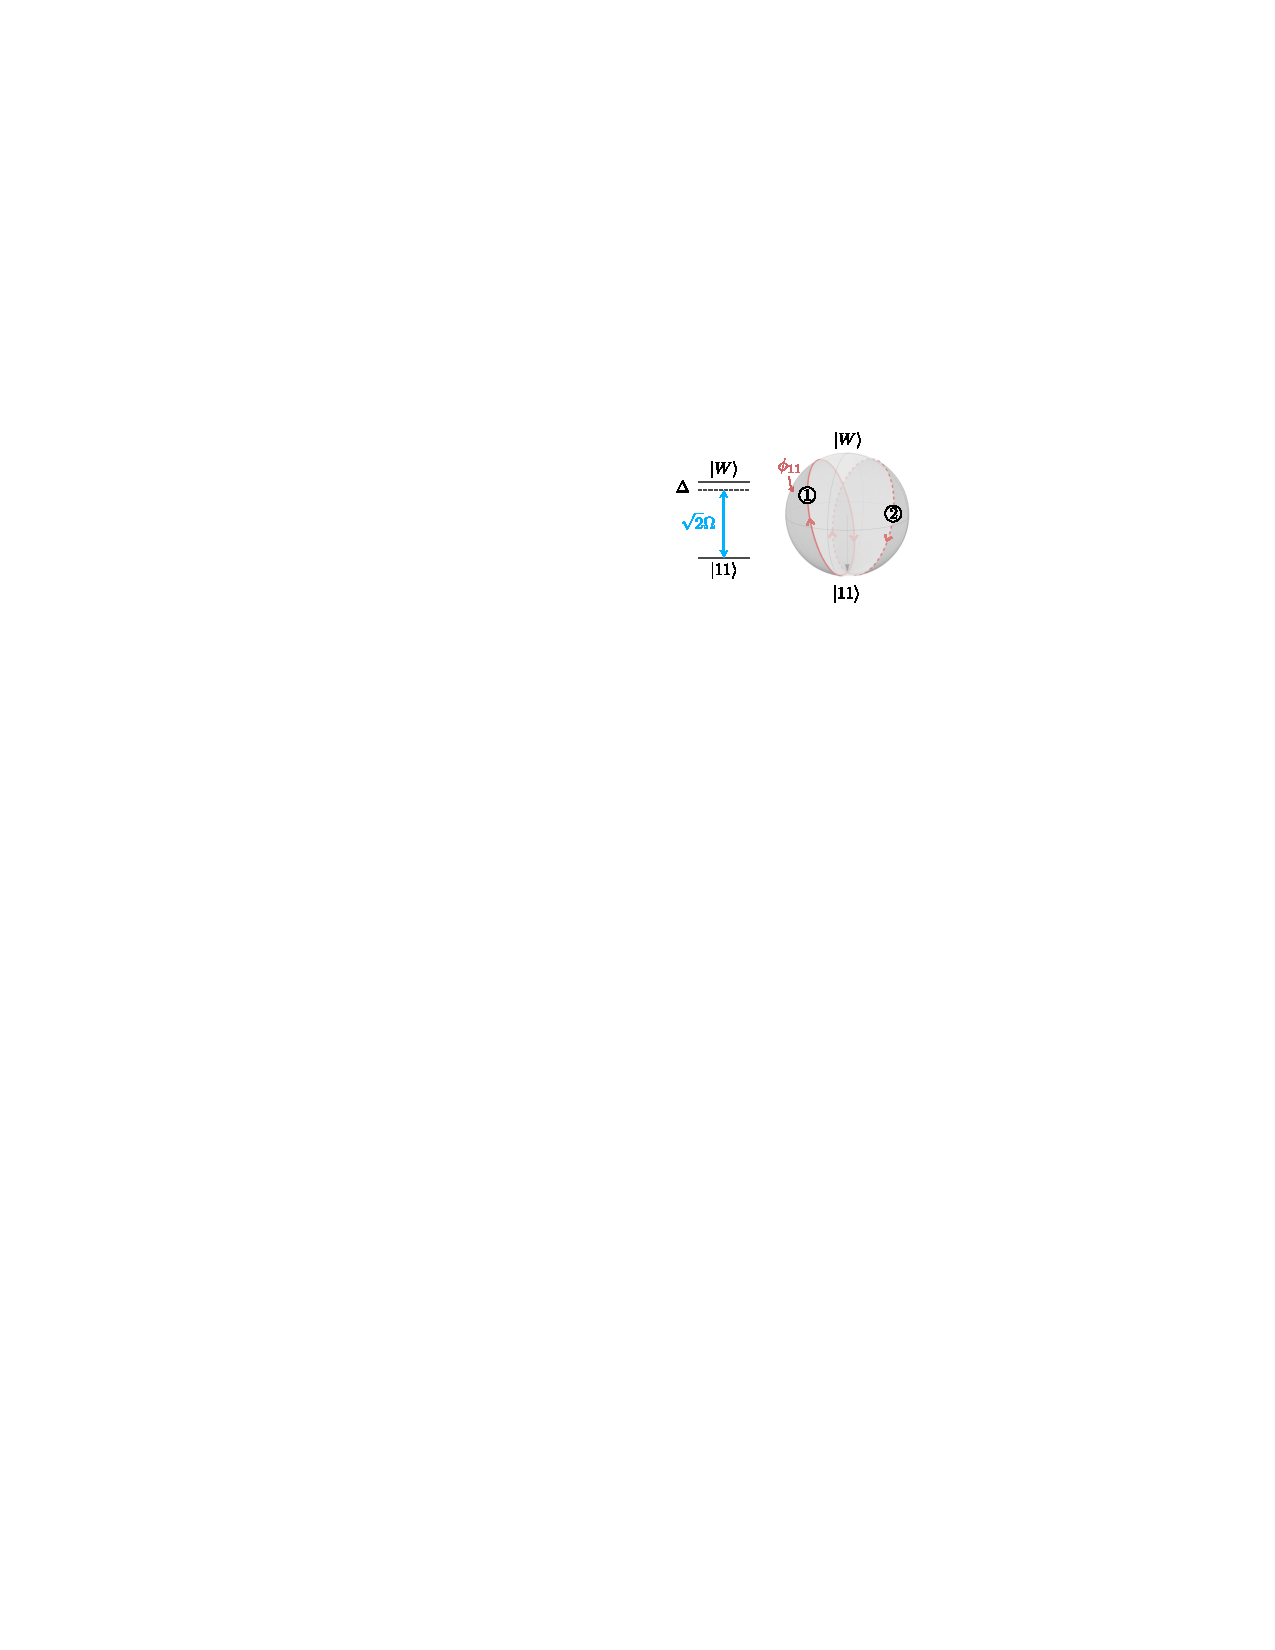
\includegraphics[width=0.4\textwidth]{image/physical_implementation/11-dynamics.pdf}  \label{fig:11-dynamics} }
    \end{minipage}
    \caption{The dynamics of $\ket{01}$ and $\ket{11}$ states can be described by two-level systems with the same detuning but different effective Rabi frequencies. For a fixed detuning, the pulse length $\tau$ is selected such that the first laser pulse drives an incomplete Rabi oscillation on the $\ket{01}$ system, while the $\ket{11}$ system undergoes a complete detuned Rabi cycle. The phase of the second pulse $xi$ is chosen such that for the $\ket{01}$ system a second pulse of length $\tau$ completes the oscillation and returns to the state $\ket{01}$. For the $\ket{11}$ system the second pulse drive a second complete cycle.}
    \label{fig:dynamics}
    \end{figure}

\clearpage

For a fixed detuning $\Delta$, the pulse length $\tau$ is chosen such that:
\begin{enumerate}
    \item the \textit{first laser pulse} drives an incomplete oscillation on the $\ket{01}$ system, while the $\ket{11}$ system completes a full cycle of a detuned Rabi oscillation;
    
    \item the driving field of the \textit{second laser pulse} is rotated around the $z$-axis by an angle $\xi$ such that a second pulse of length $\tau$ completes the oscillation for a $\ket{01}$ system returning to $\ket{01}$. It also drives a second complete oscillation on the $\ket{11}$ configuration.
\end{enumerate}

After the second pulse, both $\ket{01}$ and $\ket{11}$ systems return to their initial positions on the Bloch sphere but with an accumulated dynamical phases $\phi_{01}$ and $\phi_{11}$ (Fig. \ref{fig:dynamics}, \ref{fig:dynamical-phase}). The acquired dynamical phase depends on the solid angle enclosed by the $\Delta$-dependent trajectories on the Bloch sphere. It varies from $2\pi$ to 0 with increasing $\Delta$. Specifically, with a choice of the laser detuning as $\Delta \approx 0.377 \, \Omega$, the dynamical phase $\phi_{11}=2\phi_{01}-\pi$, which realizes the CZ gate described in Eq. \eqref{eq:CZ-gate-map}.

    \begin{figure}[h!]
    \begin{minipage}[c]{0.49\linewidth}
    \centering
    \subfloat[][Dynamical phase $\phi_{01}$. ]{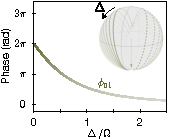
\includegraphics[width=0.5\textwidth]{image/physical_implementation/01-dynamical-phase.pdf} \label{fig:01-dynamical-phase} }
    \end{minipage}
    \begin{minipage}[]{0.49\linewidth}
    \centering
    \subfloat[][Dynamical phase $\phi_{11}$. ]{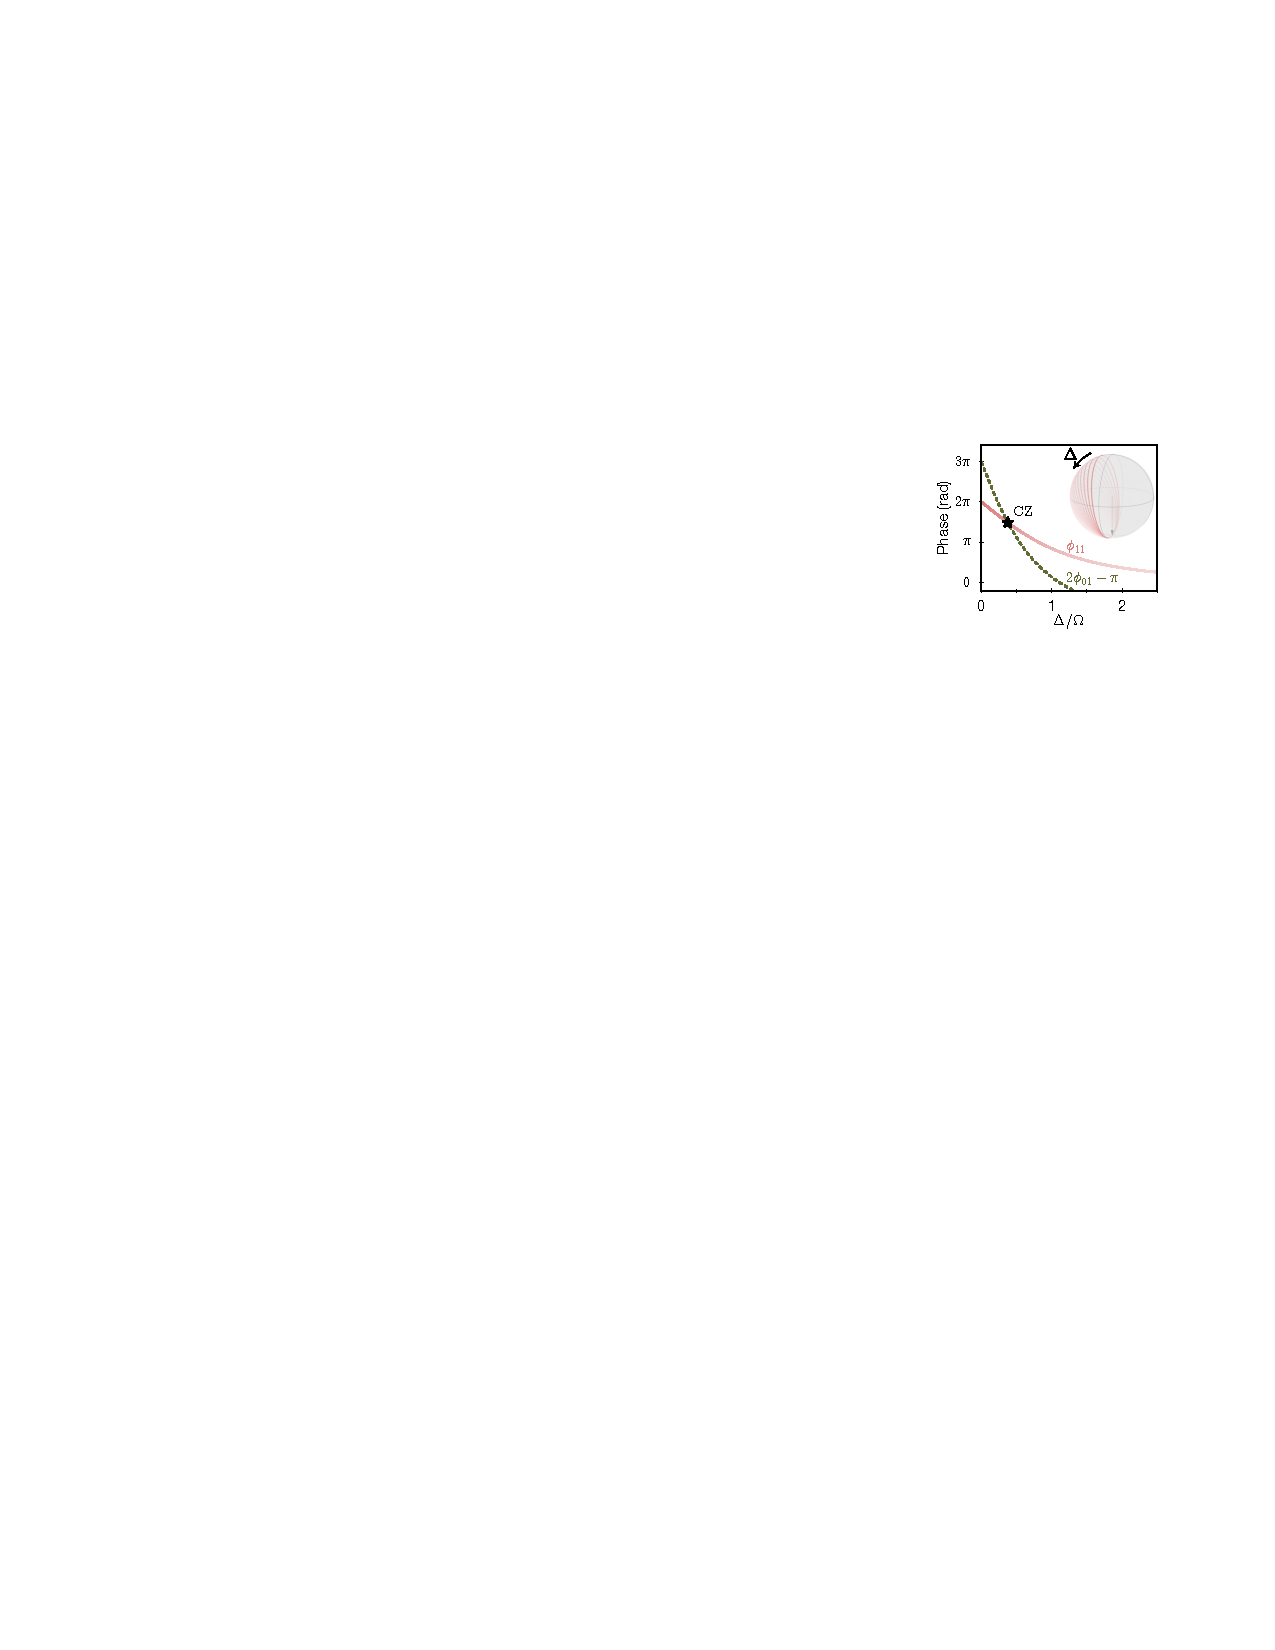
\includegraphics[width=0.5\textwidth]{image/physical_implementation/11-dynamical-phase.pdf}  \label{fig:11-dynamical-phase} }
    \end{minipage}
    \caption{The dynamical phases $\phi_{01}$ and $\phi_{11}$ are determined by the solid angle enclosed by the trajectories on the Bloch sphere (shaded area). They vary from $2\pi$ to 0 as a function of $\Delta$ corresponding to increasingly shallow trajectories. The CZ gate mapped in \eqref{eq:CZ-gate-map} is realized by choosing $\Delta \approx 0.377 \, \Omega$. }
    \label{fig:dynamical-phase}
    \end{figure}
 
\clearpage
 
\section{Theoretical design of two-qubit CZ gate}  
\label{sec:theoretical_design_CZ}
The dynamics of a two-qubit CZ gate, implemented with the protocol described in Sec. \ref{sec:physical_implementation}, is governed by the following Hamiltonian:
\begin{equation}
    H = \sum_{i=1}^{2}  \qty[ \frac{1}{2} \qty( \Omega \ket{1}_i \bra{r} +
    \Omega^* \ket{r}_i \bra{1} ) -
    \Delta \ket{r}_i \bra{r} ] +
    V \ket{r}_1 \bra{r} \otimes \ket{r}_2 \bra{r}
\end{equation}
where $\Delta$ is the detuning of the excitation laser from the transition frequency between states $\ket{1}$ and $\ket{r}$, and $\Omega$ is the Rabi frequency. $V$ is the interaction strength between two atoms in Rydberg states. 

\paragraph{Perfect blockade.} If the interaction between two atoms in Rydberg states is strong, i.e. $V \gg \abs{\Omega}, \abs{\Delta}$, the system is in the Rydberg blockade regime. The dynamics of the system simplifies as:
\begin{itemize}
    \item the state $\ket{00}$ does not evolve;
    
    \item if one of the two atoms is in $\ket{0}$, only the system in $\ket{1}$. evolves. The dynamics can be described with a two level system with states $\ket{a_1}\equiv\ket{1}$ and $\ket{b_1}\equiv\ket{r}$ and Hamiltonian:
    \begin{equation}
        H_1 = \frac{1}{2} \qty( \Omega \ket{a_1}\bra{b_1} + 
        \Omega^* \ket{b_1}\bra{a_1})
        - \Delta \ket{b_1}\bra{b_1}
        \label{eq:perfect-H_1}
    \end{equation}
    
    \item if both atoms are initially in $\ket{1}$, the dynamics can be described with a two level system with states $\ket{a_2}\equiv\ket{11}$ and $\ket{b_2}\equiv \frac{1}{\sqrt{2}} \qty( \ket{r,1} + \ket{1,r} )$ and Hamiltonian:
    \begin{equation}
        H_2 = \frac{\sqrt{2}}{2} \qty( \Omega \ket{a_2}\bra{b_2} + 
        \Omega^* \ket{b_2}\bra{a_2})
        - \Delta \ket{b_2}\bra{b_2}
        \label{eq:perfect-H_2}
    \end{equation}
    
\end{itemize}

As explained in details in Sec. \ref{sec:physical_implementation}, the CZ gate is implemented with two identical global pulses of the Rydberg laser field with equal duration $\tau$ and detuning $\Delta$ and with a phase jump by $\xi$ in between. Each pulse is mathematically represented by an unitary evolution of the state:
\begin{equation}
    U = \exp(-i H \tau)
    \label{eq:unitary_evolution}
\end{equation}
Moreover, the change of the laser phase between the two pulses is represented by a rotation by an angle $\xi$ around the $z$-axis, $\Omega \rightarrow \Omega e^{i\xi}$. Finally, the operator $\mathcal{U}$ is defined as the application of both laser pulses. 

The computational basis states evolve as follows under the action of $\mathcal{U}$:

\begin{itemize}
    \item the state $\ket{00}$ does not evolve:
            \begin{equation}
                \mathcal{U} \ket{00} = \ket{00}
            \end{equation}
       
    \item the state $\ket{11}$ evolves as:
            \begin{equation}
                \mathcal{U} \ket{11} = e^{i\phi_2} \ket{11}
                \label{eq:11-unitary-evolution}
            \end{equation}    
    where the accumulated dynamical phase is $\phi_2= 2\pi \times 2 \Delta / \sqrt{\Delta^2+2\Omega^2}$. 
    Indeed, if we select the pulse duration $\tau$ such that:
    \begin{equation}
        \tau = \frac{2\pi}{ \sqrt{\Delta^2+2\Omega^2} }
    \end{equation}
    the first laser pulse drive a complete detuned Rabi cycle for the $\ket{11}$ state, namely $U\ket{11}=e^{i\phi_2/2}\ket{11}$. The second pulse also leads to a complete Rabi cycle about a different axis, but results in the same accumulated phase. In total, we find that the evolution of the system under the application of both laser pulses is as Eq. \eqref{eq:11-unitary-evolution}.
   
    \item the states $\ket{01}$ or $\ket{10}$ evolve as:
            \begin{equation}
            \begin{aligned}
                 \mathcal{U} \ket{01} &= e^{-i\phi_1} \ket{01} \\
                 \mathcal{U} \ket{10} &= e^{-i\phi_1} \ket{10}
            \end{aligned}
            \end{equation}        
    Indeed, after the first pulse, due to the mismatch between the effective Rabi frequencies in $H_1$ and $H_2$, the state $\ket{01}$ (or $\ket{10}$) does not return to itself, but a superposition state is created:
            \begin{equation}
            \begin{aligned}
                 U \ket{01} &= \cos(\alpha) \ket{01} + \sin(\beta) e^{i\gamma} \ket{0r} \\
                 U \ket{10} &= \cos(\alpha) \ket{10} + \sin(\beta) e^{i\gamma} \ket{r0}
            \end{aligned}
            \end{equation}      
    With a proper choice of the phase jump $\xi$ between the two pulses, the system returns to the state $\ket{01}$ (or $\ket{10}$) after the second pulse.
    This proper choice is:
        \begin{equation}
        e^{-i\xi} = \frac{-
        \sqrt{(\Delta/\Omega)^2+1} \cos\qty(\frac{1}{2}\Omega\tau \sqrt{(\Delta/\Omega)^2+1}) + i\Omega\tau\sin\qty(\frac{1}{2}\Omega\tau \sqrt{(\Delta/\Omega)^2+1})
        }{
        \sqrt{(\Delta/\Omega)^2+1} \cos\qty(\frac{1}{2}\Omega\tau \sqrt{(\Delta/\Omega)^2+1}) + i\Omega\tau\sin\qty(\frac{1}{2}\Omega\tau \sqrt{(\Delta/\Omega)^2+1})
        }
        \label{eq:exp_xi}
    \end{equation}
    
\end{itemize}

Both the acquired dynamical phases $\phi_1$ and $\phi_2$ are solely determined by the dimensionless quantity $\Delta/\Omega$. Finally, a choice for $\Delta/\Omega$ can be found in order to have $\phi_2= 2\phi_1 + \pi$.
With this choice we reproduce exactly the behavior of controlled-phase gate in Eq. \eqref{eq:CZ-gate-map}.
The numerical values of the optimal parameters which describes this dynamics are:
\begin{subequations}
    \begin{align}
        \Omega\tau &= 4.29268 \label{eq:opt_val_Ot} \\
        \xi &= 3.90242 \label{eq:opt_val_xi} \\
        \Delta/\Omega &= 0.377371 \label{eq:opt_val_DO}
    \end{align}
    \label{eq:opt_val}
\end{subequations}




\paragraph{Accounting for imperfect blockade.} If finite blockade interactions are accounted for, the finite value of $V$ only affects the dynamics if the system is initially in the state $\ket{11}$. Indeed, the dynamics of a system initially in $\ket{11}$ can be described with a three level system with states $\ket{a_2}\equiv\ket{11}$, $\ket{b_2}\equiv \ket{1r}+\ket{r1}$ and $\ket{c_2}=\ket{rr}$ and Hamiltonian:
    \begin{equation}
        H_2 = \frac{\sqrt{2}}{2} \qty( \Omega \ket{a_2}\bra{b_2} + \Omega \ket{b_2}\bra{c_2} +
        \Omega^* \ket{c_2}\bra{b_2} + \Omega^*\ket{b_2}\bra{a_2}) 
        - \Delta \ket{b_2}\bra{b_2} 
        + (V-2\Delta)\ket{c_2}\bra{c_2}
        \label{eq:imperfect-H_2}
    \end{equation}
For small $V>0$ and a given $\Delta$, a value for $\Omega$ and $\tau$ can always be chosen such that a system initialized in $\ket{11}$ returns to itself after just the first pulse, as in the perfect blockade assumption. Thus in the finite blockade regime the complete Rabi oscillation are simply replaced by a slightly more complicated path, but which is still closed in the Bloch sphere.

For $V \gg \abs{\Delta},\abs{\Omega}$, the results of the perfect blockade regime are obtained. Indeed, the effect for finite blockade simply reduces to the two-level system, $\{ \ket{a_2}, \ket{b_2}\}$, where the detuning $\Delta$ is renormalized by $\Omega^2/(2V)$. 





\clearpage


\section{Code implementation of two-qubit CZ gate}
\label{sec:code_implementation}
A numerical simulation of the two-qubit CZ gate, described in details in Sec. \ref{sec:theoretical_design_CZ}, is performed. First of all, a two-qubit system is implemented in order to investigate the dynamics of a cluster of two atoms under the action of the controlled-phase gate.
Then, we implement a chain of $N$-qubit where the CZ gate is applied between consequent qubits under the assumption that there is interaction only within an atom pair. This is useful for a further analysis to study how a Gaussian noise for the optimal parameters in Eq. \eqref{eq:opt_val} propagates through the chain.

\subsection{Two-qubit system}

To simulate the dynamics of a two-qubit system under the application of the two-qubit CZ gate, the Python library QuTip is used. This library provides ready-use functions to handle quantum systems and also provide optimized solvers for time evolution of Schrödinger's equations.
The system is composed by two atoms each one can be in states $\ket{0}$, $\ket{1}$ or $\ket{r}$. Thus system state vectors have dimension $d=3^2$.

\paragraph{Perfect blockade.} Under the assumption of a perfect blockade regime, the dynamics of the system decouples into a few simple sectors described by the Hamiltonians in Eqs. \eqref{eq:perfect-H_1} and \eqref{eq:perfect-H_2}. 
The total Hamiltonian of the system, $H_{\text{CZ}}$, has dimension $3^2 \times 3^2$ and it is implemented in the Python function  {\bfseries\texttt{hamiltonian}}\texttt{(Omega,Delta)}.
The CZ gate is implemented in function  {\bfseries\texttt{CZ$\_$gate}}\texttt{(psi,Omega,Delta,tau)}. In more details, the time between 0 and $\tau$ is discretized and each pulse is applied to the system as a unitary evolution (Eq. \eqref{eq:unitary_evolution}). In particular, the second pulse is rotated by $\Omega \rightarrow \Omega^{i\xi}$. The unitary evolution of the system state is calculated using the QuTiP function {\bfseries\texttt{qutip.mesolve}}. It evolves the state vector in the list of times, using an ordinary differential equation solver. Using this function, also expectation values for a set of operator can be evaluated in time.

\begin{lstlisting}[style=myPython]
# Hamiltonian definition
def hamiltonian(Omega,Delta):
    
    H0  = 0 * tensor(psi00.dag(),psi00)
    
    H01 = 1/2 * ( Omega*tensor(psi01.dag(),psi0r) + np.conj(Omega)*tensor(psi0r.dag(),psi01) ) 
        - Delta*tensor(psi0r.dag(),psi0r)
    
    H10 = ...
    H2  = ...

    H = H0 + H01 + H10 + H2
    
    return H
\end{lstlisting}

\begin{lstlisting}[style=myPython]
# CZ gate implementation
def CZ_gate(psi,Omega,Delta,tau):
        
    # Times discretization
    times = np.linspace(0.0, tau, 200)
    
    # Apply first pulse 
    H = hamiltonian(Omega,Delta)
    result = mesolve(H, psi, times,[], [])
    psi = result.states[-1]
    
    # Apply second pulse rotated by Omega -> Omega exp(i xi)
    H = hamiltonian(Omega * exp_xi(Delta,Omega,tau), Delta)
    result = mesolve(H, psi, times,[], [])
    psi = result.states[-1] 
        
    return result
\end{lstlisting}

 
\paragraph{Imperfect blockade.} If finite blockade interactions are taken into account, only the dynamics of the system initially in $\ket{11}$ is affected and the Hamiltonian for this sector becomes as in Eq. \eqref{eq:imperfect-H_2}. The total Hamiltonian is implemented in the function {\bfseries\texttt{hamiltonian$\_$imperfect}}\texttt{(Omega,Delta,V)}. The dynamics of the system is simulated with the QuTip function {\bfseries\texttt{qutip.mesolve}} as for the perfect Rydberg blockade case.



\subsection{Chain of N-qubit}
\label{subsec:chain-N-qubit}

\begin{figure}[H]
\fontsize{10pt}{12pt}\selectfont
    \begin{minipage}[t]{0.6\linewidth}\setlength{\parindent}{9pt}

We implement a numerical simulation of a chain of $N$-qubit where the CZ gate is applied between consequent qubits, assuming perfect blockade regime.
Physically, it is like considering a one-dimensional array of atoms where, each time the two-qubit CZ gate acts on a pair of atoms, the interaction with the other atoms is neglected.
In order to obtain the behavior of the map in Eq. \eqref{eq:CZ-gate-map} between the first and last qubits, they can be initialized either in state $\ket{0}$ or $\ket{1}$, while all the other qubits in the chain are initialized in $\ket{0}$. 

The state vector of the $N$-qubit system is computed as the tensor product of the subsystems as:
\begin{equation}
    \ket{\psi} = \ket{q_1} \otimes \dots \otimes \ket{q_N}
\end{equation}

    \end{minipage}
    \hfill
    \begin{minipage}[t]{0.37\linewidth} \vspace{-0.5cm}
    \centering
\begin{equation*}
\Qcircuit @C=0.8em @R=1.1em {
\lstick{\ket{1}_0}	& \ctrl{1}	& \qw      & \qw & \qw &\qw & \qw            & \qw & \qw & \qw & \qw & \qw & \qw\\
\lstick{\ket{0}_1}	& \gate{Z}	& \ctrl{1} & \qw & \qw &\qw & \qw            & \qw & \qw & \qw & \qw & \qw & \qw\\
\lstick{\dots}	    & \qw 	    & \gate{Z} & \qw & \qw &\qw & \qw            & \qw & \qw & \qw & \qw & \qw & \qw\\
                    &           & \vdots   &     &  \vdots   &    &    & \vdots     &     &     &     &     &    \\
\lstick{\dots}      & \qw	    & \qw      & \qw & \qw &\qw & \qw       & \qw & \qw & \qw & \ctrl{1} & \qw & \qw\\
\lstick{\ket{1}_N}	& \qw	    & \qw      & \qw & \qw &\qw & \qw       & \qw & \qw & \qw & \gate{Z}& \qw & \qw\\
}
\end{equation*}
    \caption{Circuit scheme of CZ gate in a chain of $N$-qubit.}
    \label{fig:chain-CZ-circuit}
    \end{minipage}
\end{figure}

The function {\bfseries\texttt{chain$\_$init}} \texttt{(N,state$\_$first,state$\_$last)} computes the initial state of the chain, given the initial state of the first and the last qubits. Then, in the function {\bfseries\texttt{chain\_CZ\_gate}}\texttt{(psi,Omega,Delta,tau,method,niter)} the CZ gate in a chain of $N$-qubit is implemented. 
Starting from the first qubit, we apply the two-qubit CZ gate iteratively. In the $i$-th iteration, the total Hamiltonian of the chain, $H_{chain} \in 3^N\times 3^N$, let evolve the $i$-th and the $(i+1)$-th qubits without affecting the remaining $N-2$. It is computed as:
\begin{equation}
    H_{chain,i}^{(N)} =  \underbrace{\mathbb{I}_3  \otimes \dots \otimes \mathbb{I}_3}_{i-1} \otimes H_{\text{CZ}} \otimes \underbrace{ \mathbb{I}_3  \otimes \dots \otimes \mathbb{I}_3}_{N-i-1}.
\end{equation}

\begin{lstlisting}[style=myPython]
# Chain state initialization
def chain_init(N,state_first,state_last):
    
    psi = basis(3,state_first) 
    for i in range(N-2):
        psi = tensor(psi,basis(3,0))
    psi = tensor(psi,basis(3,state_last))

    return psi
\end{lstlisting}

\begin{lstlisting}[style=myPython]
# Chain CZ-gate function
def chain_CZ_gate(psi,Omega,Delta,tau,method,niter):

    N = len(dims(psi)[0]) # Number of qubits in the chain
    I = qeye(3) # Define identity matrix
    Hp1 = Qobj( hamiltonian(Omega,Delta) ) # First pulse hamiltonian
    Hp2 =  Qobj( hamiltonian(Omega * exp_xi(Delta,Omega,tau), Delta) ) # Second pulse hamiltonian 
    times = np.linspace(0.0, tau, niter) # Discretize time
        
    for i in range(N-1):
        
        mat_list1 = [I]*(N-1)
        mat_list2 = [I]*(N-1)
        mat_list1[i] = Hp1
        mat_list2[i] = Hp2
        
        H1 = mat_list1[0]
        H2 = mat_list2[0]
        
        for i in range(N-2):
            H1 = tensor(H1,mat_list1[i+1])
            H2 = tensor(H2,mat_list2[i+1])
        
        result = mesolve(H1, psi, times,[], [])
        psi = result.states[-1]
        result = mesolve(H2, psi, times,[], [])
        psi = result.states[-1]
    
    return psi
\end{lstlisting}

\clearpage

\section{Numerical methods for time-dependent Schr{\"o}dinger equation solvers}
\label{sec:numerical_methods_time_evolution}
For the $N$-qubit system discussed in Sec. \ref{subsec:chain-N-qubit}, as longer chains are considered, the dimension of the total Hamiltonian of the system scales as $3^N \times 3^N$.
Given the Hamiltonian $H$ of the system, the time-dependent Schrödinger equation can be solved as:
\begin{equation}
    \ket{\psi(t)} = U(t) \ket{\psi(0)}, \qquad U(t)=e^{-iHt/\hbar}
    \label{eq:time-evolution}
\end{equation}
The time evolution of the system can become computationally challenging for large $N$.
Therefore, we consider several time-dependent Schr{\"o}dinger solvers, along with some optimizations, in order to test their performances. We implement these algorithms using different coding environment and libraries implementation both on CPU and GPU. 

\paragraph{Numpy implementation}
First of all, we implement a script analogous to the one described in Sec. \ref{subsec:chain-N-qubit}, but based on NumPy and SciPy Python libraries. Numpy provides support for large, multi-dimensional arrays, along with a collection of high-level mathematical functions to operate on these arrays. In particular, NumPy is coded in well-optimized C code, so it allows to exploit the flexibility of Python and the speed of compiled code. It guarantees generally faster execution time compared to Python built in types. SciPy integrates and expand Numpy tools providing additional functions to operate with matrices, as well as sparse array libraries. Eventually, NumPy, along with SciPy, supports a wide range of hardware and computing platforms and plays well with parallel computing. 

\paragraph{Tensorflow implementation} 
Then, we implement again the code using TensorFlow, a Python library for machine learning, which is optimized to deal with large matrices and in particular can be easily executed on GPU thanks to CUDA. 

\paragraph{Fortran implementation}
Finally, the same code is implemented using Fortran programming language. Indeed, it is most of the most powerful language for scientific computation with LAPACK routines for linear algebra. The design of Fortran allows the compiler to perform stronger optimizations. 


\subsection{Spectral method}
\label{subsec:spectral-method}
We compute the unitary time evolution of the system as in Eq. \eqref{eq:time-evolution}. To do this, we first diagonalize the system Hamiltonian with the decomposition $H = PDP^{-1}$, where $D$ is the diagonal matrix and $P$ is the eigenvectors matrix.
Its exponential can be computed as:
\begin{equation}
    e^{-iHt} = P e^{-iDt} P^{-1}
\end{equation}
This method requires the computation of eigenvalues and eigenvectors of a matrix and the inversion of a matrix.

In Numpy, we implement the function {\bfseries\texttt{spectral\_evol}} \texttt{(H, psi, tau)} in which the eigenvalues decomposition is achieved through the function {\bfseries\texttt{numpy.linalg.eigh}}, optimized for complex Hermitian matrices, which is implemented using \texttt{\_syevd} and \texttt{\_heevd} LAPACK routines for computing eigenvalues and eigenvectors, respectively. The inversion of the matrix is achieved through the function {\bfseries\texttt{numpy.linalg.inv}} which again relies on LAPACK routines. 

\begin{lstlisting}[style=myPython]
# Time evolution with spectral method in Numpy
def spectral_evol(H, psi, tau):

    eiglist = np.linalg.eigh(H)
    eigenvalues = eiglist[0]
    eigenvectors = eiglist[1]
    eigenvectors_inv = np.linalg.inv(eigenvectors)
    
    exp_diag = np.diag(np.exp(-1j*eigenvalues*tau))

    exp_H = np.dot(eigenvectors,np.dot(exp_diag,eigenvectors_inv))
    
    return np.dot(exp_H,psi)
\end{lstlisting}

In TensorFlow, the unitary time evolution operator is computed by means of the function {\bfseries\texttt{tensorflow.linalg.expm}} to compute the exponential matrix.

Finally, in Fortran, implementation eigenvalues decomposition is achieved through {\bfseries\texttt{\_heev}} and the matrix inversion is obtained with {\bfseries\texttt{\_getrf}} and {\bfseries\texttt{\_getri}} LAPACK routines based on LU decomposition.

\subsection{Crank-Nicolson method}
\label{subsec:crank-nicolson}
The time evolution of the system is also performed using Crank-Nicolson algorithm. Given a discrete time step $\Delta t$, the unitary time evolution operator ca be written as:
\begin{equation}
    e^{-iH\Delta t} = e^{-\frac{iH\Delta t}{2}} e^{-\frac{iH\Delta t}{2}} = \qty( e^{\frac{iH\Delta t}{2}} )^{-1} e^{-\frac{iH\Delta t}{2}}
    \simeq  \qty( 1 + \frac{iH\Delta t}{2} )^{-1} 
    \qty( 1 - \frac{iH\Delta t}{2} ) + O(\Delta t)^3
\end{equation}
Thus the time evolved wave function can be computed as
\begin{equation}
    \psi(x,t+\Delta t) = 
    \qty( 1 + \frac{iH\Delta t}{2} )^{-1} 
    \qty( 1 - \frac{iH\Delta t}{2} ) \psi(x,t).
\end{equation}.
This is equivalent to solve the linear system:
\begin{equation}
    \qty( 1 + \frac{iH\Delta t}{2} )    \psi(x,t+\Delta t) = \qty( 1 - \frac{iH\Delta t}{2} ) \psi(x,t).
\end{equation}
By iterating the procedure $n_{iter}$ times, we obtain the time evolution for time $T = \Delta t \times n_{iter}$.

In Numpy, the Crank-Nicolson method is implemented in the function {\bfseries\texttt{crank\_nicolson}}\texttt{(H, psi, tau, n\_iter)}. Given the Hamiltonian, it computes the time evolution of the initial state $\psi$ for a time $\tau$ using $n_{iter}$ iterations. In this algorithm we need to solve a linear system of equations. To do this we exploit the function {\bfseries\texttt{numpy.linalg.solve}} which uses LAPACK routine \texttt{\_gesv}. 

\begin{lstlisting}[style=myPython]
# Crank-Nicolson solver in Numpy
def crank_nicolson(H, psi, tau, n_iter):
    
    time = np.linspace(0, tau, n_iter)
    dt = time[1] - time[0]
    
    A = np.eye(H.shape[0], dtype=data_type) + 1j * H * dt/2
    B = np.eye(H.shape[0], dtype=data_type) - 1j * H * dt/2

    b = np.dot(B,psi) 

    for i in time:
        
        psi = np.linalg.solve(A, b)
        b = np.dot(B,psi) 
        
    return psi  
\end{lstlisting}

For TensorFlow implementation we write an analogous function using {\bfseries\texttt{tensorflow.linalg}} module.
 
\subsection{Crank-Nicolson method with LU decomposition} 
\label{subsec:crank-nicolson-lu}
In order to optimize Crank-Nicolson algorithm we consider the LU decomposition method for solving linear systems. 
Indeed, an invertible matrix $A$ can be decomposed into two factors $LU$, where $L$ is a lower and a $U$ an upper triangular matrix. Thus the linear system $A\boldsymbol{x} = \boldsymbol{y}$ can be recasted as: 
\begin{equation}
    \begin{cases}
        L\boldsymbol{z} = \boldsymbol{y} \\
        U\boldsymbol{x} = \boldsymbol{z} \\
    \end{cases}
\end{equation}
In our case the matrix $A$ is fixed and the system has to be solved many times for different $\boldsymbol{x}$ and $\boldsymbol{y}$, so this procedure is convenient because we can execute the LU decomposition just once. Then, to solve the systems only two back substitutions are required.

In Numpy, we define the function {\bfseries \texttt{crank\_nicolson\_LU}}\texttt{(H, psi, tau, n\_iter)}. Again, given the Hamiltonian, it computes the time evolution of the initial state $\psi$ for a time $\tau$ using $n_{iter}$ iterations.
We compute the LU decomposition through {\bfseries\texttt{scipy.linalg.lu}} function and we solve the systems we exploiting the {\bfseries\texttt{scipy.linalg.solve\_triangular}} function optimized for triangular matrices. 

\begin{lstlisting}[style=myPython]
# Crank-Nicolson LU optimized solver in Numpy
def crank_nicolson_LU(H, psi, tau, n_iter):
    
    time = np.linspace(0, tau, n_iter)
    dt = time[1] - time[0]
    
    A = np.eye(H.shape[0], dtype=data_type) + 1j * H * dt/2
    B = np.eye(H.shape[0], dtype=data_type) - 1j * H * dt/2

    b = np.dot(B,psi) 
    
    L, U = scipy.linalg.lu(A, permute_l = True)

    for i in time:
        
        y = scipy.linalg.solve_triangular(L,b,lower=True)
        psi = scipy.linalg.solve_triangular(U,y,lower=False)        
        b = np.dot(B,psi) 
    
    return psi
\end{lstlisting}

As before, for TensorFlow implementation we write an analogous function using {\bfseries\texttt{tensorflow.linalg}} module.

Finally, we can observe that the total Hamiltonian of the $N$-qubits system is a \textit{sparse matrix}. Therefore, we optimize the Crank-Nicolson algorithm with LU decomposition for the case of sparse matrices. We implement the function {\bfseries\texttt{crank\_nicolson\_LU\_sparse}} \texttt{(H, psi, tau, n\_iter)} which is analogous to  {\bfseries\texttt{crank\_nicolson\_LU}}. Now, the matrices are transformed into \texttt{csc\_matrix} sparse matrices and optimized functions are used for LU decomposition and triangular systems solving. Instead, no sparse matrix optimized solvers are provided with TensorFlow. 








\clearpage

\section{Results}

%Finally to test the results we implement a function to compute the fidelity between two states. In particular, we consider that we are dealing with pure quantum states so we compute the fidelity as:
%\begin{equation}
%    F(\psi,\phi) = \abs{\bra{\psi}\ket{\phi}}^2
%\end{equation}

The behavior of the CZ gate, described theoretically in Sec. \ref{sec:theoretical_design_CZ}, is numerically simulated as explained in Sec. \ref{sec:code_implementation}. Firstly, we analyze the CZ gate acting on a two-qubit system in both the perfect and imperfect blockade regime. The correctness of the simulation is verified by fixing the optimal parameters (Eq. \eqref{eq:opt_val}) and comparing the results with the experimental one discussed in Sec. \ref{sec:physical_implementation}. Then, we vary the optimal parameters in order to investigate the behavior of the CZ gate in response to this variation. After that, the measurement process is simulated by introducing a Gaussian noise on the parameters in the case of perfect and imperfect blockade regime.
Then, we consider CZ gate in the case of a chain of $N$-qubit. Again, a Gaussian noise is introduced on the optimal parameters to investigate noise effects with an increasing number of qubits.
Finally, a timing analysis of the several algorithms for time evolution and implementations, discussed in Sec. \ref{sec:numerical_methods_time_evolution}, is performed. 

\subsection{CZ gate in a two-qubit system}

Let us consider a system of two-qubit with the CZ gate acting between them. In more details, the system is composed by two atoms each one can be in states $\ket{0}$, $\ket{1}$ and $\ket{r}$. The dynamics is analyzed both in the case of perfect blockade regime or finite blockade interactions. 

\subsubsection{Correct behaviour check and optimal parameters variation}

\paragraph{Perfect blockade.} As explained in details in Sec. \ref{sec:physical_implementation} and \ref{sec:theoretical_design_CZ}, under the assumption of a perfect Rydberg blockade, the dynamics of the states $\ket{01}$ (or $\ket{10}$) and $\ket{11}$ can be simplified as the one of a two-level system with same detuning $\Delta$ and different Rabi frequencies. In particular, the Rabi frequency of $\ket{01}$ (or $\ket{10}$) is $\Omega$, while the one of $\ket{11}$ has an enhanced Rabi frequency $\sqrt{2}\Omega$, as one can see by comparing the Eqs. \eqref{eq:perfect-H_1} and \eqref{eq:perfect-H_2}. More specifically, the dynamics, under the application of the first pulse of duration \eqref{eq:opt_val_Ot}, is simulated in Fig. \ref{fig:population_perfect-blockade} for different $\Delta/\Omega$ ratios. If the system is initially in the state $\ket{01}$ (or $\ket{10}$), only the atoms that it is in $\ket{1}$ evolves and oscillates between the states $\ket{a_1}\equiv\ket{1}$ and $\ket{b_1}\equiv\ket{r}$ (Fig. \ref{fig:population_01}). 
One can note that for null detuning (blue line) the oscillation of the quantum system is most efficient. In this case, the population inversion oscillates between -1 and +1. For the ratio chosen as optimal parameters in Eq. \eqref{eq:opt_val_DO} (orange line), the amplitude of the oscillation is slightly reduced. Then, for an extreme value of $\Delta/\Omega$, we note that the oscillations have an high frequency. If the system is initially in the state $\ket{11}$, then the dynamics is again equivalent to that of an effective two-level system formed by the states $\ket{a_2}\equiv\ket{11}$ and $\ket{b_2}\equiv \frac{1}{\sqrt{2}} \qty( \ket{r,1} + \ket{1,r} )$.

\begin{figure}[h!]
\begin{minipage}[c]{0.49\linewidth}
\subfloat[][Dynamics of $\ket{01}$.]{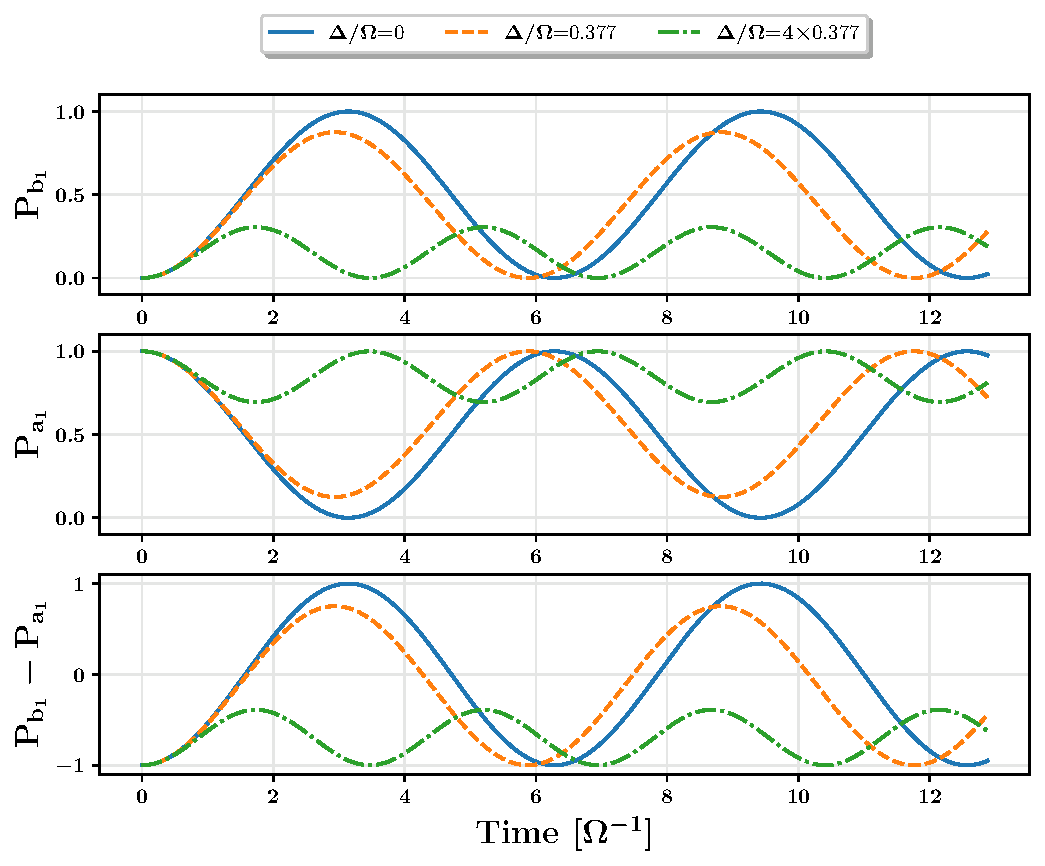
\includegraphics[width=1.0\textwidth]{image/two-qubit-system/pop_H1.pdf} \label{fig:population_01} }
\end{minipage}
\begin{minipage}[]{0.49\linewidth}
\centering
\subfloat[][Dynamics of $\ket{11}$.]{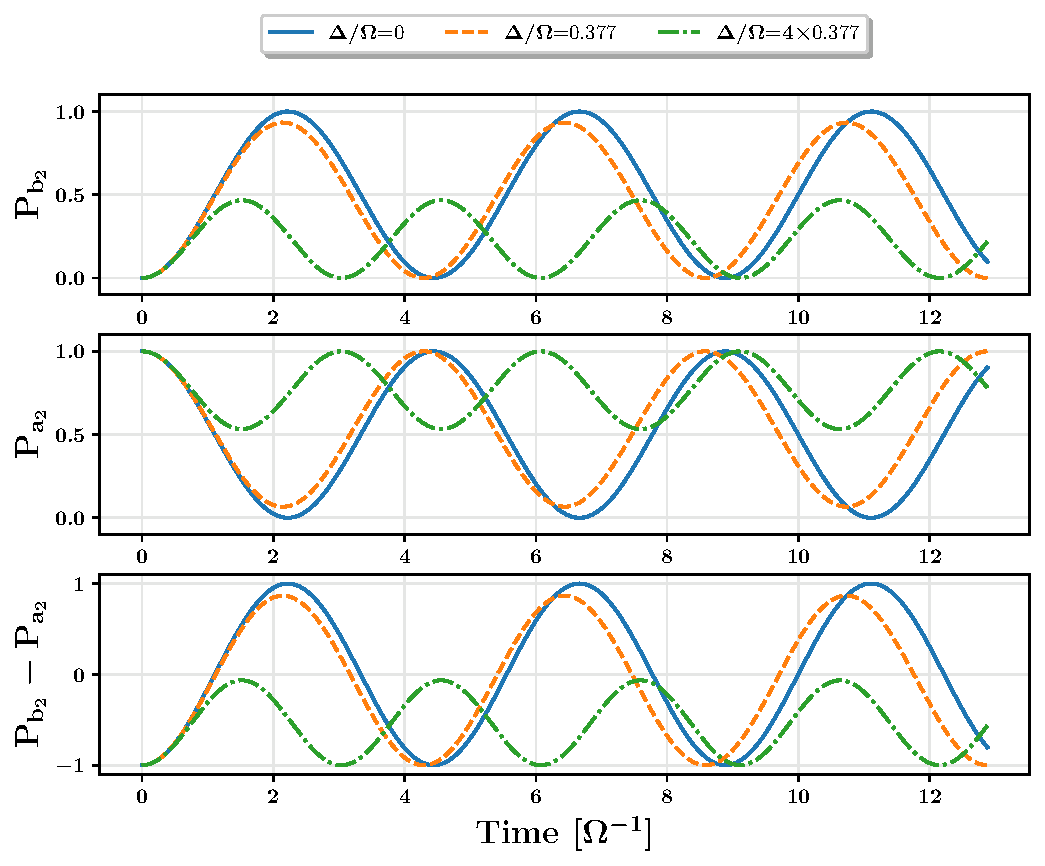
\includegraphics[width=1.0\textwidth]{image/two-qubit-system/pop_H2.pdf}  \label{fig:population_11} }
\end{minipage}
\caption{Time-dependence of the populations and the inversion for the two-level systems in Eqs. \eqref{eq:perfect-H_1} and \eqref{eq:perfect-H_2} under Rydberg perfect blockade assumption for different $\Delta/\Omega$ ratios. The duration of the pulse is fixed by the product $\Omega \tau = 4.293$ (Eq. \eqref{eq:opt_val_Ot}). }
\label{fig:population_perfect-blockade}
\end{figure}


Moreover, the duration of the pulse $\tau$ is chosen such that the state $\ket{11}$ evolve as Eq.  \eqref{eq:11-unitary-evolution} after the two pulses, i.e. it return to itself and acquire a dynamical phase $\phi_{11}$. Then, the proper choice of the phase jump between the two pulses $\xi$ as in Eq. \eqref{eq:exp_xi} guarantees that the system initially in $\ket{01}$ return to itself after the second pulse (the same for $\ket{10}$) with a dynamical phase $\phi_{01}$.
Finally, there is a proper choice for $\Delta/\Omega$ such that $\phi_{11}=2\phi_{01}-\pi$, in order to realize a controlled-phase gate up to a global gauge rotation.
The phase evolution as a function of the $\Delta/\Omega$ ratio is plotted in Fig. \ref{fig:phase_perfect-blockade}. This behavior resemble exactly what we have already shown in Fig. \ref{fig:dynamical-phase}. Thus, the CZ gate behaves correctly as expected from the theory discussed in Sec. \ref{sec:theoretical_design_CZ} by choosing the optimal parameters in \eqref{eq:opt_val}. 

\begin{figure}[H]
\begin{minipage}[c]{0.49\linewidth}
\subfloat[][Phase of $\ket{01}$ (or $\ket{10}$).]{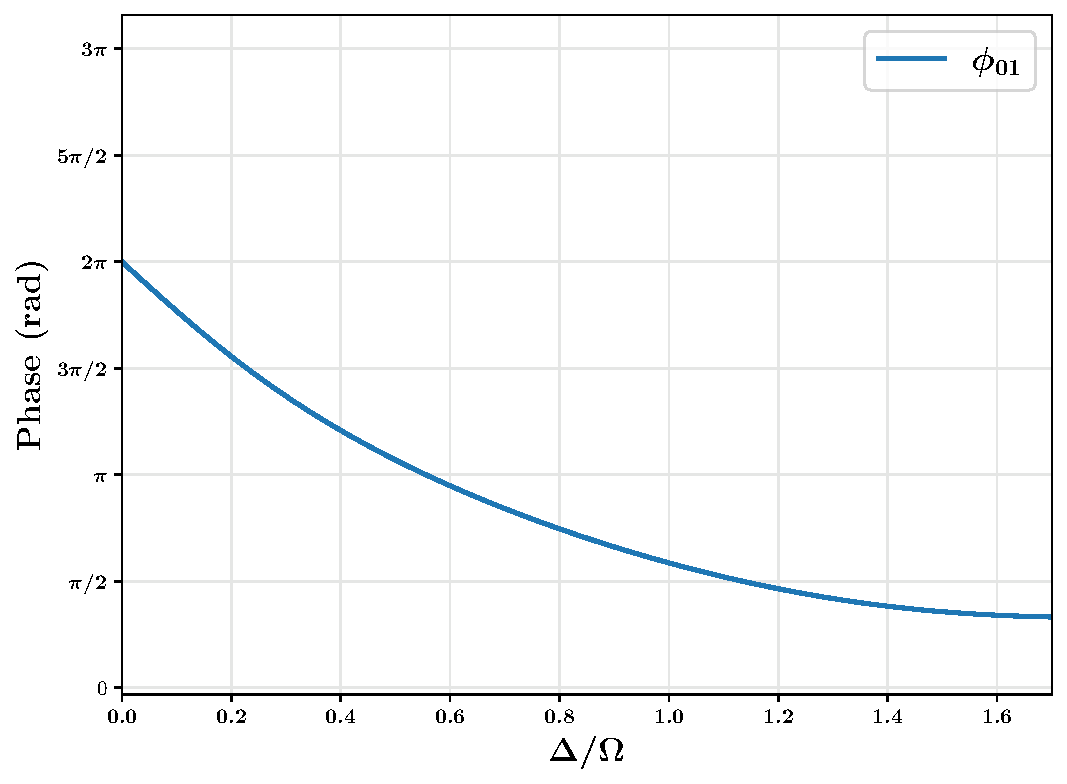
\includegraphics[width=1.0\textwidth]{image/two-qubit-system/phase_01_CZ.pdf} \label{fig:phase_01_CZ} }
\end{minipage}
\begin{minipage}[]{0.49\linewidth}
\centering
\subfloat[][Phase of $\ket{11}$.]{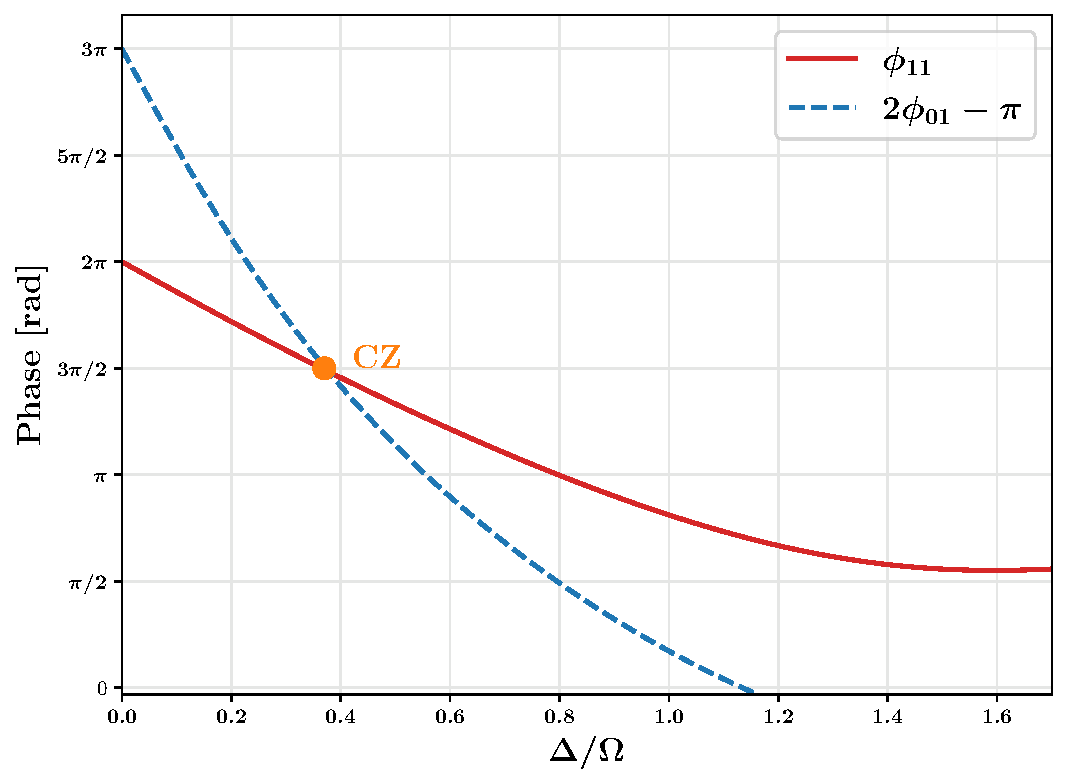
\includegraphics[width=1.0\textwidth]{image/two-qubit-system/phase_11_CZ.pdf}  \label{fig:phase_11_CZ} }
\end{minipage}
\caption{Dynamical phase $\phi_{01}$ (or $\phi_{10}$) and $\phi_{11}$ acquired respectively by the states $\ket{01}$ (or $\ket{10}$) and $\ket{11}$ after the application of the two pulses. The intersection between $\phi_{11}$ and $2\phi_{01}-\pi$ shown in \ref{fig:phase_11_CZ} realizes the CZ gate. }
\label{fig:phase_perfect-blockade}
\end{figure}

After verifying the correctness of the CZ gate implementation, we vary the optimal parameters in order to investigate the behavior of the controlled-phase gate in different conditions.
As already said in details, the key point for a controlled-phase gate implementation is that, after the application of the two pulses, a system initially in $\ket{01}$ (or $\ket{10}$) and $\ket{11}$ return to itself with an acquired dynamical phase. To estimate the error on the state of the system, we perform fidelity measurements. More specifically, we will refer as \textit{error} to the following quantity:
\begin{equation}
    \epsilon \equiv 1 - F(\rho_{init},\rho_{fin})
    \label{eq:epsilon_fidelity}
\end{equation}
where $F$ is the fidelity between the initial $\rho_{init}$ and final state $\rho_{fin}$.
Moreover, we compute the phase of the final state to monitor its value. 

First of all, the quantity $\Omega \tau$ is changed and the error $\epsilon$ is measured. 
If the system is initially in $\ket{01}$ (or $\ket{10}$) the error remains approximately null as a function of $\Omega \tau$.
Indeed, in this case, the state return to itself with a very low error regardless $\Omega\tau$. However, the dynamical phase $\phi_{01}$ acquired is still influenced by this choice. Instead, the result for a pair of atom initially in $\ket{11}$ is shown in Fig. \ref{fig:figure_merit_Omega_tau}. One can note a peak of $\epsilon=0.5$ between $2<\Omega \tau<4$. Another peak is present between $6<\Omega \tau<8$. Hence, the optimal parameter choice is in between the two peaks. Thus, we can conclude that an optimal choice for $\Omega \tau$ is required in order to implement a CZ gate correctly.
For the sake of completeness, in the same plot also the evolution of the dynamical phase $\phi_{11}$ is shown. 

Then, we vary the quantity $\Delta/\Omega$ in order to investigate the response of the system. In Fig. \ref{fig:figure_merit_Delta_Omega}, the error $\epsilon$, for a system initially in $\ket{11}$, is plotted as a function of this ratio. Also the dynamical phase $\phi_{11}$ is shown. One can note that the error is approximately null in a range of low detuning values. It increases monotonically as $\Delta/\Omega$ is growing.  
Again, if the system is initially in $\ket{01}$ (or $\ket{10}$), the error $\epsilon$ remains approximately null. Instead, as before, the dynamical phase $\phi_{01}$ is strongly influenced by this ratio as already shown in Fig. \ref{fig:phase_01_CZ}.


\begin{figure}[H]
\begin{minipage}[c]{0.49\linewidth}
\subfloat[][$\Omega\tau$ variation.]{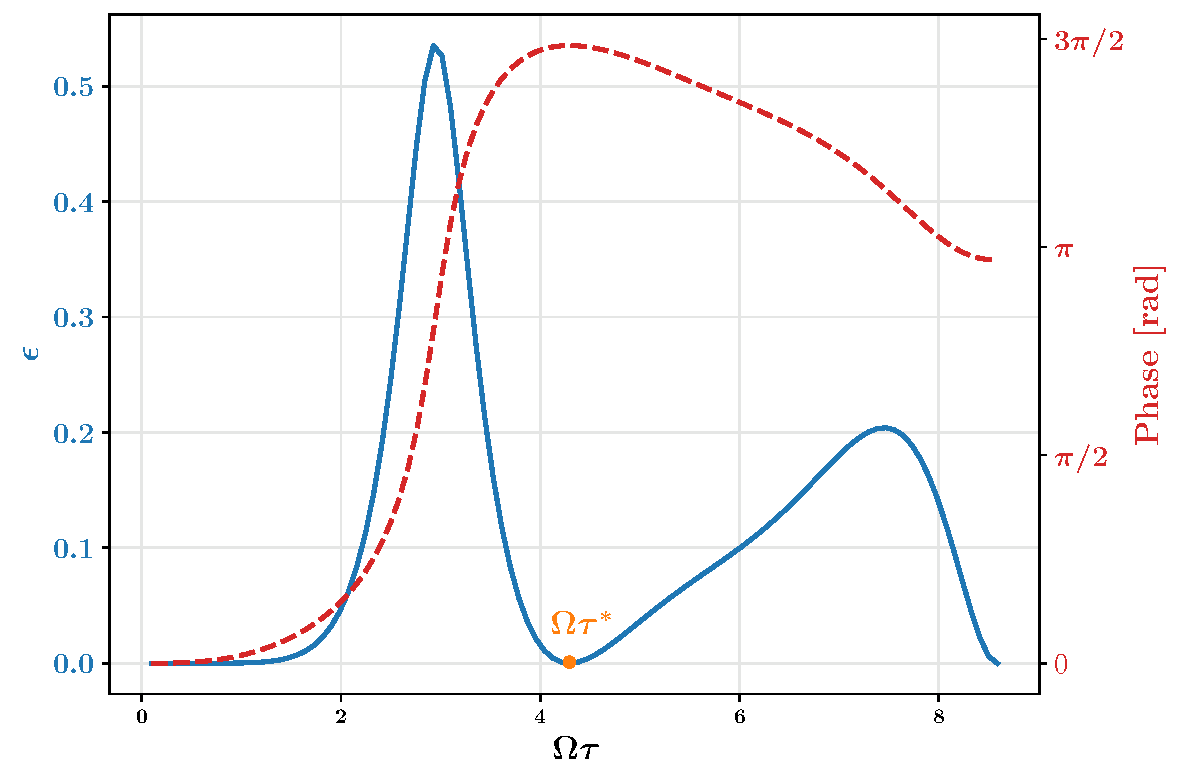
\includegraphics[width=1.0\textwidth]{image/two-qubit-system/epsilon-phase_omega-tau.pdf} \label{fig:figure_merit_Omega_tau} }
\end{minipage}
\begin{minipage}[]{0.49\linewidth}
\centering
\subfloat[][$\Delta/\Omega$ variation.]{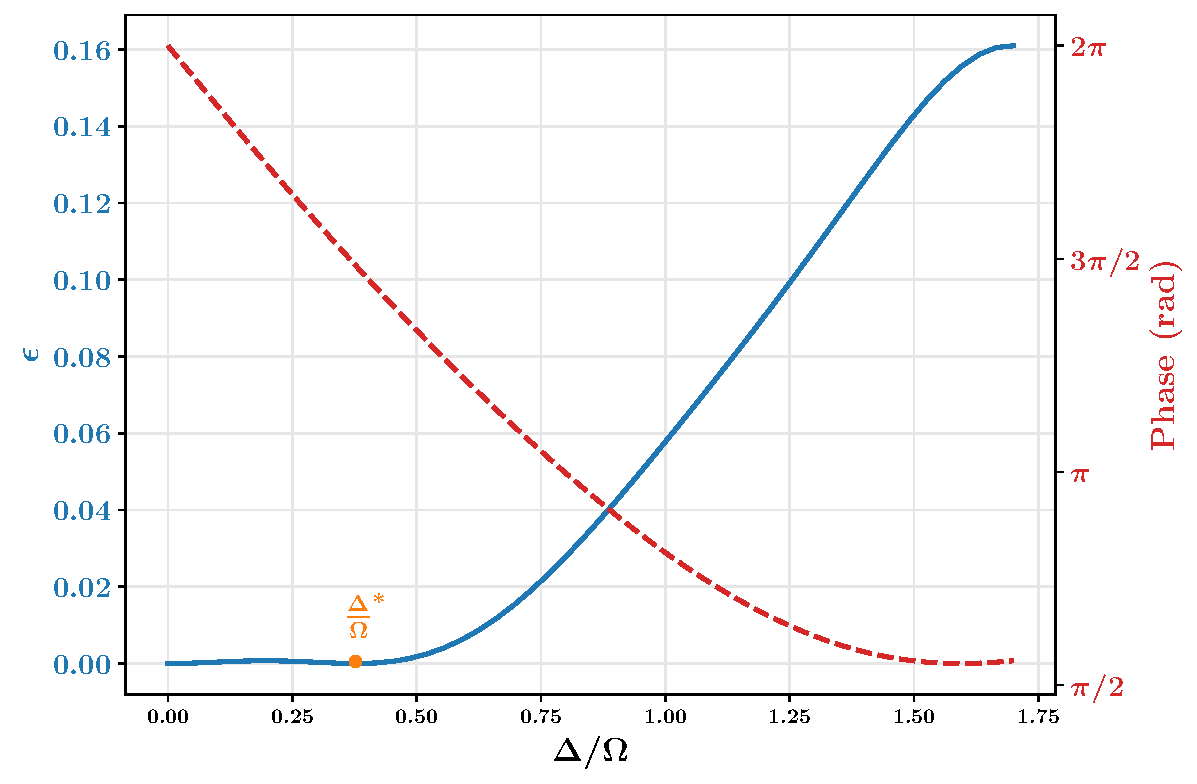
\includegraphics[width=1.0\textwidth]{image/two-qubit-system/epsilon-phase_delta-omega.pdf}  \label{fig:figure_merit_Delta_Omega} }
\end{minipage}
\caption{In blue, the error computed as in Eq. \eqref{eq:epsilon_fidelity} for a system initially in state $\ket{11}$ is plotted as a function of $\Omega\tau$ and $\Delta/\Omega$ in \ref{fig:figure_merit_Omega_tau} and \ref{fig:figure_merit_Delta_Omega} respectively.  In red, also the dynamical phase $\phi_{11}$ acquired by the state $\ket{11}$ after the two pulses is reported. }
\label{fig:figure_merit}
\end{figure}





\paragraph{Imperfect blockade.} As already explained in Sec. \ref{sec:theoretical_design_CZ}, finite blockade interactions only affects the dynamics if the system is initially in the state $\ket{11}$. More specifically, in this case the dynamics is equivalent to that of a three-level system with states $\ket{a_2}\equiv\ket{11}$, $\ket{b_2}\equiv \ket{1r}+\ket{r1}$ and $\ket{c_2}=\ket{rr}$ and can be described by the Hamiltonian in Eq. \eqref{eq:imperfect-H_2}. In Fig. \ref{fig:population_imperfect-blockade} the time-dependence of the population, for a pair of atoms initially in $\ket{11}$ and for different values of the strength parameters $V$, is reported. One can note that, for low values of $V$, the system oscillates between the states $\ket{a_2}$, $\ket{b_2}$ and $\ket{c_2}$ as expected. Instead, already for $V=100$, the effect for finite blockade simply reduces to the two-level system with oscillations only between the states $\ket{a_2}$ and $\ket{b_2}$. In Fig. \ref{fig:phase_imperfect-blockade}, the dynamical phases $\phi_{01}$ and $\phi_{11}$ are plotted as a function of $\Delta/\Omega$ for $V=1$. As the dynamics of the $\ket{01}$ (or $\ket{10}$) state is not affected by the finite blockade interactions, the phase $\phi_{01}$ scales as already shown in Fig. \ref{fig:phase_01_CZ}. 
On the other hand, $\phi_{11}$ behaves differently and is characterized by several discontinuities. That is on account of phase computation which is periodic with a period of $2\pi$. In the plot \ref{fig:phase_imperfect-blockade}, we unwrap artificially the dynamical phase $\phi_{11}$.  
Hence, also in the case of finite blockade interactions, one can use $\Delta$ as a control knob for the relative dynamical phases acquired by $\ket{11}$ and $\ket{01}$, and thus realize a CZ gate.

\begin{figure}[H]
\begin{minipage}[c]{0.49\linewidth}
\subfloat[][Population of $\ket{11}$.]{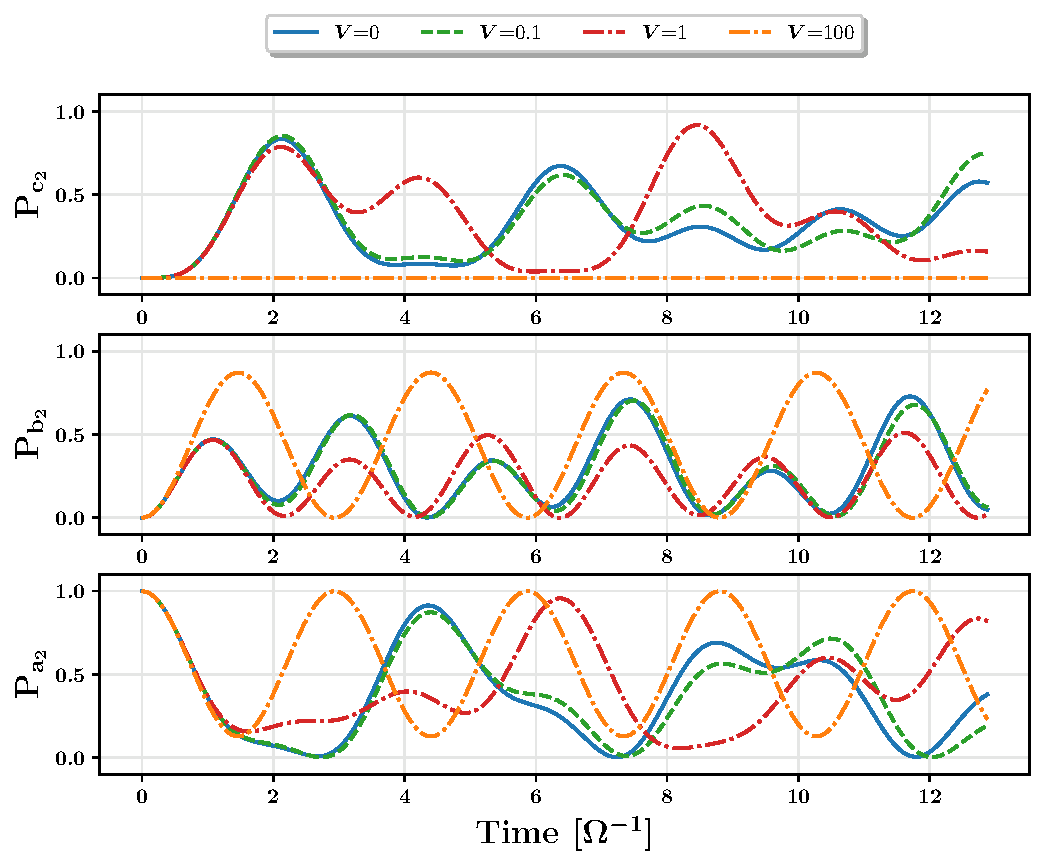
\includegraphics[width=1.0\textwidth]{image/two-qubit-system/pop_H2-imp.pdf} \label{fig:population_imperfect-blockade} }
\end{minipage}
\begin{minipage}[]{0.49\linewidth} \vspace{0.5cm}
\centering
\subfloat[][Dynamical phase of $\ket{01}$ and $\ket{11}$ for $V=1$.]{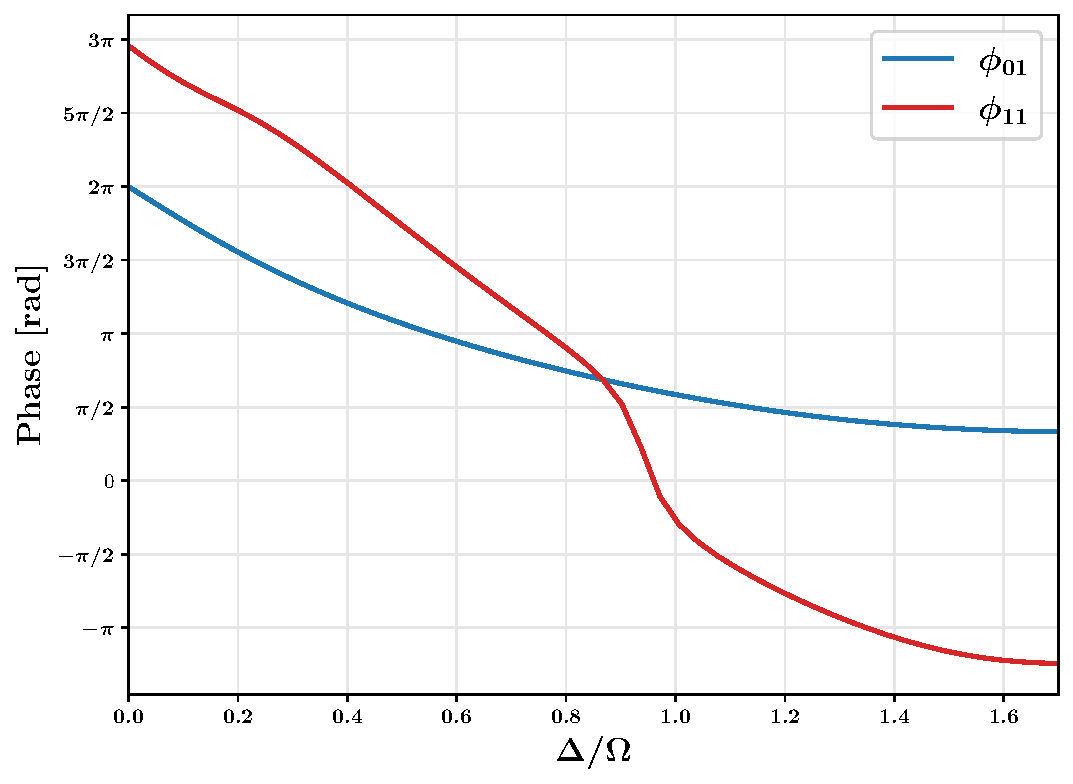
\includegraphics[width=1.0\textwidth]{image/two-qubit-system/phase_11_01_CZ_imp.pdf}  \label{fig:phase_imperfect-blockade} }
\end{minipage}
\caption{In \ref{fig:population_imperfect-blockade}, the time-dependence of the population for the three-level system in Eq. \eqref{eq:imperfect-H_2} under finite blockade interactions assumption is reported. The parameters fixed for the simulation are the one in \eqref{eq:opt_val}. In \ref{fig:phase_imperfect-blockade}, the dynamical phase of states in $\ket{01}$ (or $\ket{10}$) and $\ket{11}$ is illustrated for $V=1$ as a function of the $\Delta/\Omega$ ratio. }
\label{fig:population_phase_imperfect_blockade}
\end{figure}


\subsubsection{Measurement process with Gaussian noise on $\tau$ and $\Delta$}

Let us consider a pair of atoms initially in the state $\ket{11}$. Under the assumption of a random perturbation on the optimal parameters, we want to investigate what are the possible states allowed after the application of the CZ gate and with which probability they can be found in a measurement process.

To do this, we fix the optimal parameters as in \eqref{eq:opt_val} and we introduce a Gaussian noise with zero mean and a standard deviation of $1\%$ on both the quantities $\Omega \tau$ and $\Delta/\Omega$. Then, the CZ gate is applied and the wave-function of the final state is stored.
The experiment is ran several times ($\sim 10^3$) with these stochastic fluctuation. 
For each of the final states obtained, the measurement process is simulated: a random configuration is selected according to their probabilities. In particular, we take $10^4$ measurements for each wave-function. All the results are grouped in order to obtain enough statistics.

\paragraph{Perfect blockade} If perfect blockade assumption holds, the dynamics of the system initially in $\ket{11}$ is simulated according to the Hamiltonian in Eq. \eqref{eq:perfect-H_2}. In Fig. \ref{fig:measurement_perfect-blockade}, we show the bar plot of the measurement process simulation explained above. The system with a random perturbation of $1\%$ return with an high probability to its initial state $\ket{11}$. However, there is also a small probability to find the states $\ket{1r}$ or $\ket{r1}$.
One can also note that the final state $\ket{rr}$ is not allowed as expected. 

\begin{figure}[H]
    \centering
    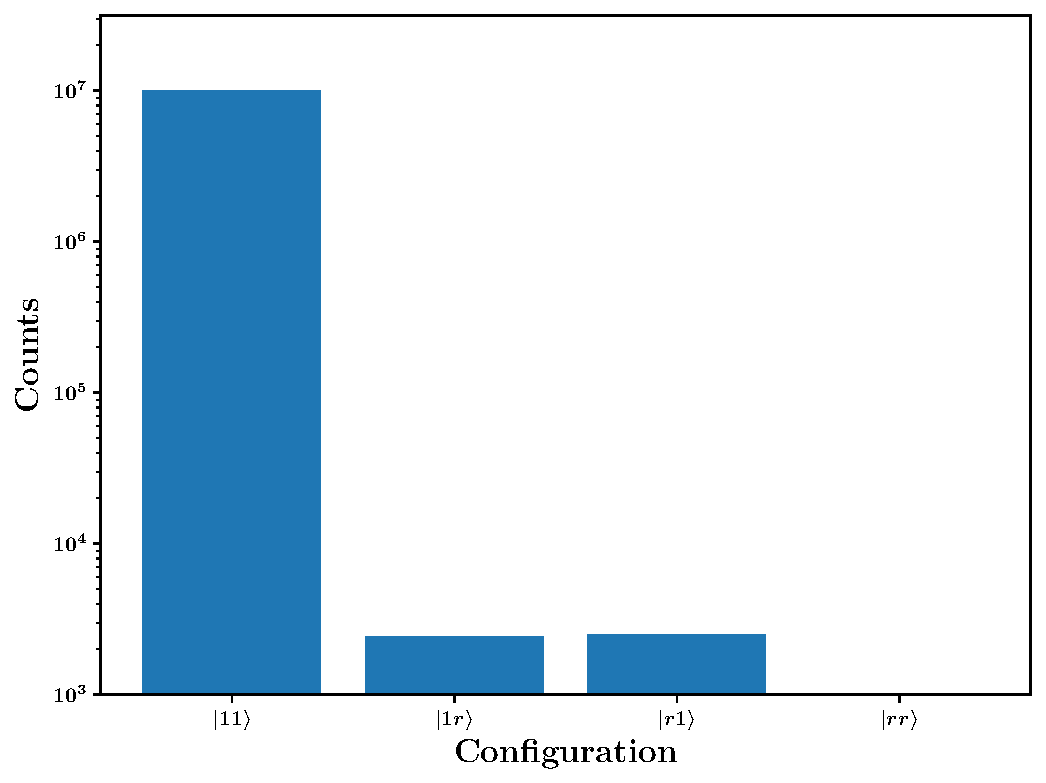
\includegraphics[width=0.5\textwidth]{image/two-qubit-system/measurement/noise_measurement_two-qubit.pdf}
    \caption{Bar plot of measurement process simulation for a system initially in $\ket{11}$ under the application of the CZ gate in perfect blockade assumption. A Gaussian noise with mean zero and standard deviation of $1\%$ is introduced on the quantities $\Omega\tau$ and $\Delta/\Omega$. The experiment is ran $10^3$ times and for each final wave-function $10^4$ measurements are taken.}
    \label{fig:measurement_perfect-blockade}
\end{figure}

\paragraph{Imperfect blockade.} Under the assumption of imperfect blockade, the system initially in $\ket{11}$ evolves according to Eq. \eqref{eq:imperfect-H_2}. 
In this case, for small values of the interaction strength parameter $V>0$, we do not know the exact values of the optimal parameters to realize the CZ gate. However, by fixing the same parameters of \eqref{eq:opt_val}, the measurement process is simulated and plotted in Fig \ref{fig:measurement_V=1}. It is interesting to note that now the state $\ket{rr}$ is allowed. Indeed, for $V=1$ the states $\ket{11}$ and $\ket{rr}$ can be measured more or less with equal probability. 

Now, let us consider the case $V\gg\abs{\Delta},\abs{\Omega}$.
As suggested by \cite{PhysRevLett.123.170503}, for big values of the strength parameter the dynamic is equivalent to the one of a two level system providing that $\Delta$ is renormalized by an amount $\Omega^2/(2V)$.
In Fig. \ref{fig:measurement_V=100}, the measurement process is simulated for $V=100$. One can note that, in this case the state $\ket{rr}$ is allowed but with a very low probability, comparable to the one of states $\ket{1r}$ and $\ket{r1}$. Hence, in the limit $V\rightarrow \infty$ we expect that the counts of the $\ket{rr}$ configuration becomes approximately null.

\begin{figure}[H]
\begin{minipage}[c]{0.49\linewidth}
\subfloat[][V=1]{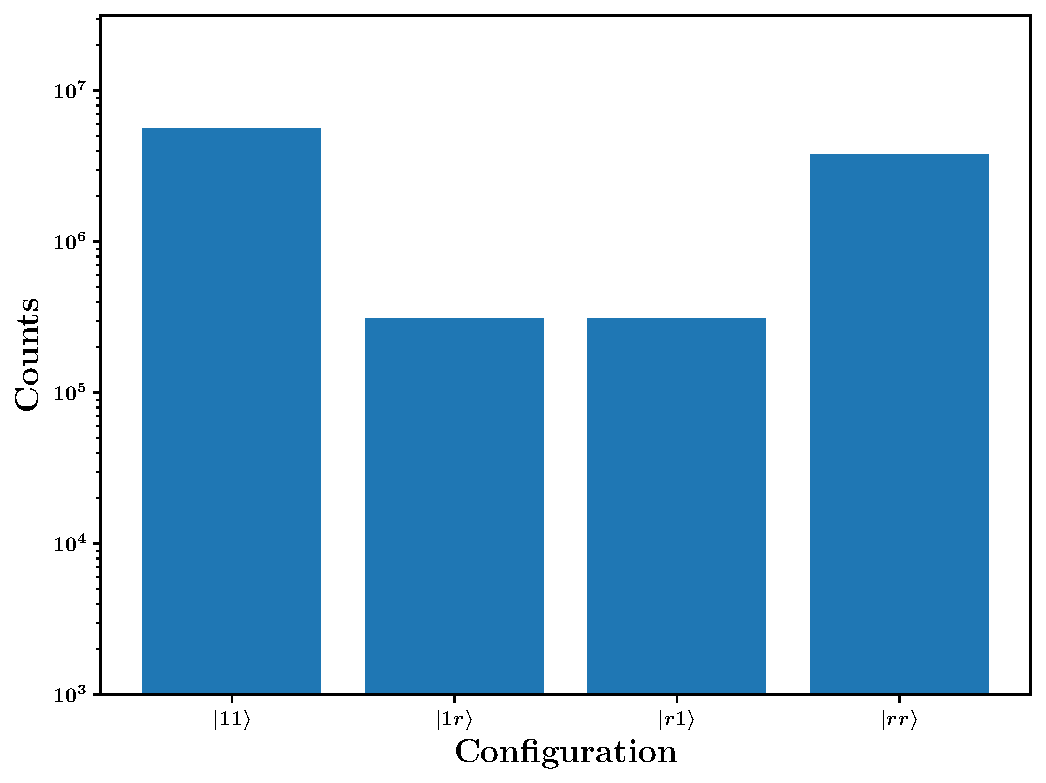
\includegraphics[width=1.0\textwidth]{image/two-qubit-system/measurement/noise_measurement_two-qubit_imp_Vlow.pdf} \label{fig:measurement_V=1} }
\end{minipage}
\begin{minipage}[]{0.49\linewidth}
\centering
\subfloat[][V=100]{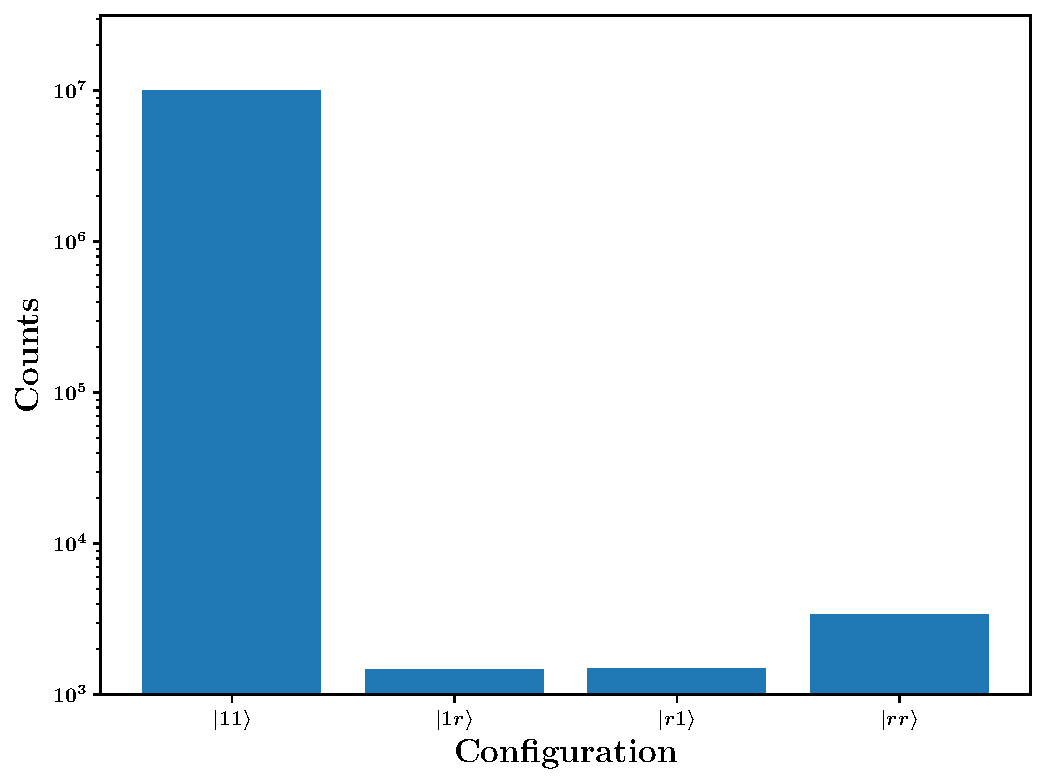
\includegraphics[width=1.0\textwidth]{image/two-qubit-system/measurement/noise_measurement_two-qubit_imp_Vbig.pdf}  \label{fig:measurement_V=100} }
\end{minipage}
\caption{Bar plot of measurement process simulation for a system initially in $\ket{11}$ under the application of the CZ gate in imperfect blockade assumption. A Gaussian noise with mean zero and standard deviation of $1\%$ is introduced on the quantities $\Omega\tau$ and $\Delta/\Omega$. The experiment is ran $10^3$ times and for each final wave-function $10^4$ measurements are taken.}
\label{fig:measurement_imperfect-blockade}
\end{figure}


\subsection{CZ gate in a chain of N-qubit}

Under the assumption of perfect blockade regime, we make a numerical simulation of a chain of $N$-qubit to investigate noise effects on the CZ gate implementation with an increasing number of qubits. In particular, the chain is implemented as explained in Sec. \ref{sec:code_implementation} and it is initialized such that both the first and the last qubits are in state $\ket{1}$. 
A Gaussian noise with zero mean and standard deviation $\sigma$ is introduced on the optimal parameters before the application of each pulse.

\begin{figure}[H]
\begin{minipage}[c]{0.49\linewidth}
\subfloat[][$\Omega \tau$]{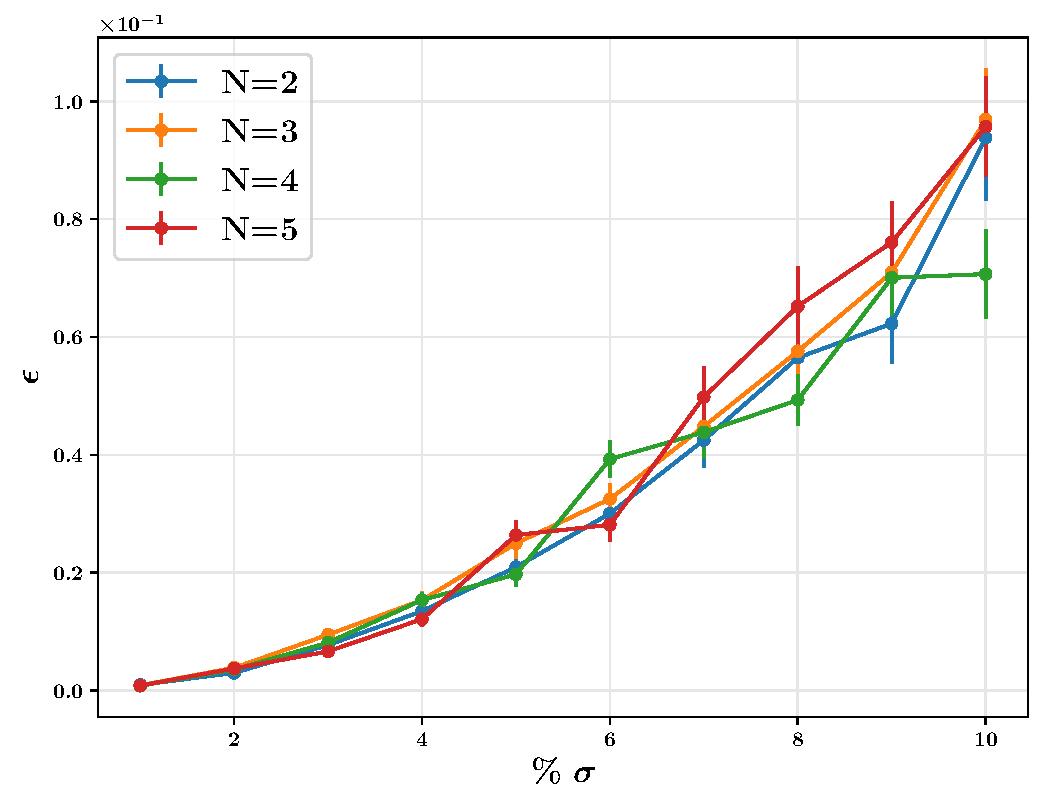
\includegraphics[width=1.0\textwidth]{image/two-qubit-system/chain/chain_sigma_tau.pdf} \label{fig:chain_tau} }
\end{minipage}
\begin{minipage}[]{0.49\linewidth}
\centering
\subfloat[][$\Delta/\Omega$]{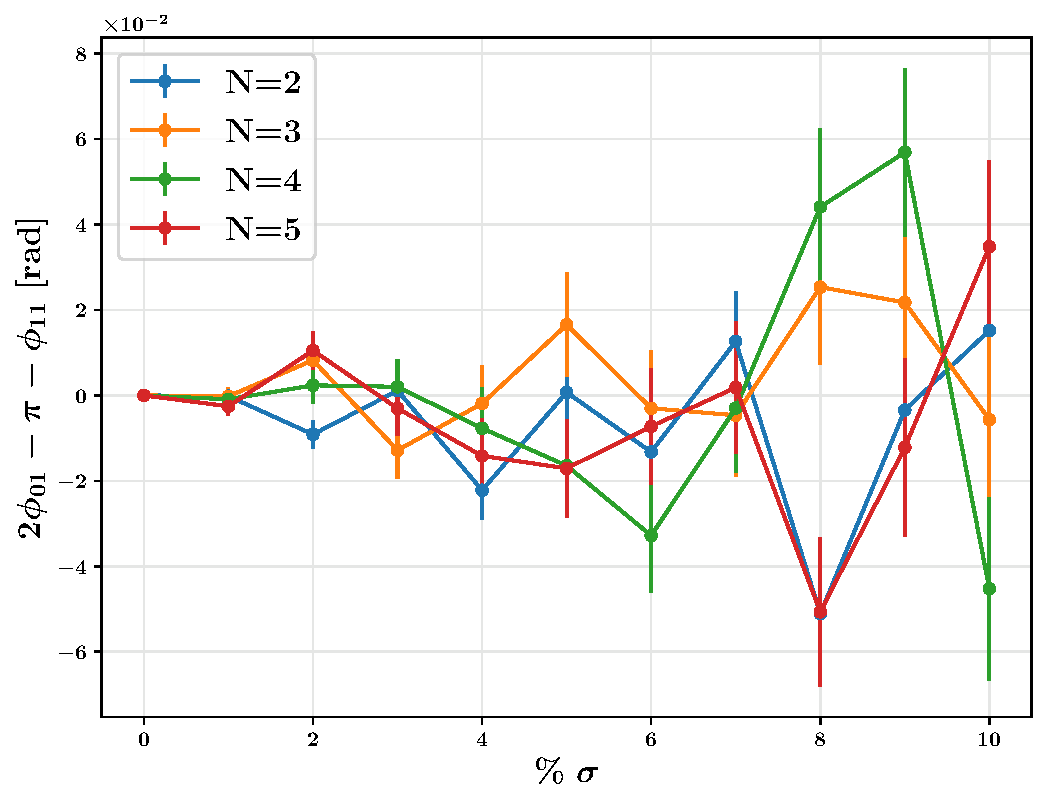
\includegraphics[width=1.0\textwidth]{image/two-qubit-system/chain/chain_phase_sigma_delta.pdf}  \label{fig:chain_delta} }
\end{minipage}
\caption{Noise effects on the CZ gate implementation in a $N$-qubit chain. A Gaussian noise with zero mean and standard deviation $\sigma$ is introduced on $\Omega\tau$ and $\Delta/\Omega$ and the result is illustrated respectively in \ref{fig:chain_tau} and \ref{fig:chain_delta}. In particular, $\% \, \sigma$ refers to the value of the standard deviation as a percentage of the optimal parameters. 
The error $\epsilon$ in \ref{fig:chain_tau} and the phase difference in \ref{fig:chain_delta} are computed as the mean of 100 iterations.}
\label{fig:chain_results}
\end{figure}


\paragraph{Gaussian noise on $\Omega \tau$} First of all, we study how a Gaussian noise on the duration of the pulse affects the dynamics. More specifically, we compute the error $\epsilon$ of the final state (defined as in Eq. \eqref{eq:epsilon_fidelity}) as a function of the noise percentage $\% \, \sigma$ of the optimal parameter for $\Omega \tau$. In Fig. \ref{fig:chain_tau}, the results for a number of qubits up to 5 and for a standard deviation up to $10\%$ are shown. We note no significant trend for a different number of qubits in the chain. Instead, we observe that increasing the value of the standard deviation of the Gaussian noise the error of the final states increases super-linearly. 


\paragraph{Gaussian noise on $\Delta/\Omega$} Then, the Gaussian noise is introduced in the detuning parameter. As already discussed, fixing the optimal parameter $\Omega\tau$ the state $\ket{11}$ return to itself. Instead, by changing $\Delta/\Omega$, the phase of the state is affected. 
The CZ gate is correctly implemented if the relation $2 \phi_{01} - \pi - \phi_{11} = 0$ holds. So, in Fig. \ref{fig:chain_delta} we study how the noise affects this relation.
Overall, one can note that a noise up to $10\%$ does not affect significantly the dynamics. Indeed, the phase difference increases with the noise but still remains approximately null ($\sim 10^{-2}$). As before, there is no significant trend increasing the number of qubits in the chain. 



\subsection{Timing analysis of time evolution methods}
 
To compare the performances of different time evolution algorithms and of different implementations discussed in Sec. \ref{sec:numerical_methods_time_evolution}, we perform a timing analysis. For this analysis, we set $\Omega$, $\Delta$ and $\tau$ accordingly to optimal parameters in Eq. \eqref{eq:opt_val} and we use a 64-bit/8-byte complex type representation (4-byte for real part and 4-byte for imaginary part).

First of all, we analyze the error $\epsilon$ of the state $\ket{11}$ and its dynamical phase as a function of the number of iterations for Crank-Nicolson methods. To this purpose, the NumPy implementation with Crank-Nicolson method with LU decomposition is used. In Fig. \ref{fig:fid_phase}, we observe that both error and phase curves stabilizes to the expected values for a number of iterations above about 100. Analogous results are obtained for other implementations and methods. Therefore, we choose 100 iterations as optimal value to obtain shorter running time and accurate results. 

\begin{figure}[H]
    \centering
    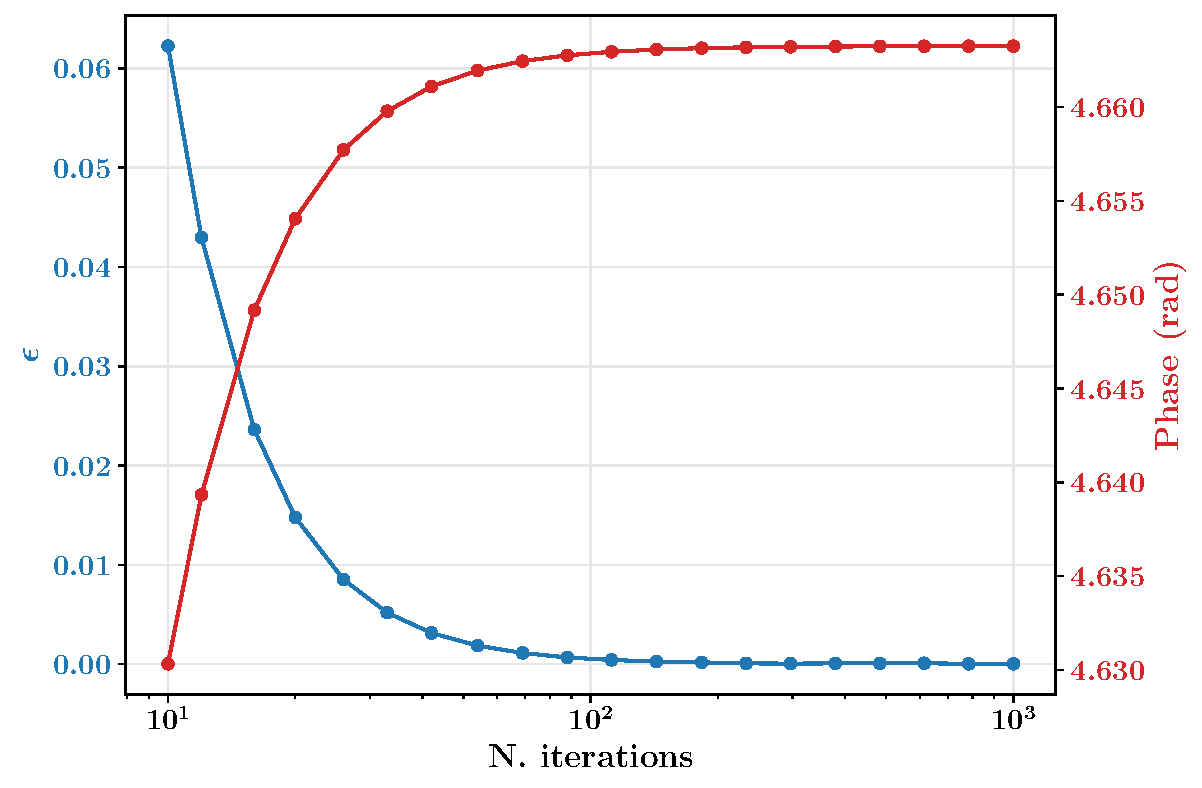
\includegraphics[width=0.6\textwidth]{image/timing/numpy_iter_fidelity_phase.pdf}
    \caption{Phase and error of state $\ket{11}$ as a function of the number of iterations for two-qubits CZ gate. We consider NumPy implementation with Crank-Nicolson with LU decomposition method.}
    \label{fig:fid_phase}
\end{figure}

Then, the elapsed time for all methods for NumPy implementation and for TensorFlow implementation (both on CPU and GPU) is measured as a function of the number of qubits $N$ in the chain. We compute the mean time over 10 realizations and we use JobLib Python library to parallelize the execution over multiple core of the CPU.

In Fig. \ref{fig:tensor_CPU}, \ref{fig:tensor_GPU} and \ref{fig:numpy}, we observe that in general Spectral Method (SM) have good performances for a small number of qubits, comparable with the Crank-Nicolson algorithm. However, its behavior highlight the fact that for a larger number of qubits the diagonalization of big matrices becomes soon unfeasible. Moreover, one can note that Crank-Nicolson algorithm with LU decomposition (CN LU) scales slower with respect to Crank-Nicolson algorithm (CN), as anticipated in Sec. \ref{subsec:crank-nicolson-lu}.
Furthermore, in Fig. \ref{fig:numpy}, we see that sparse matrix optimization guarantees a gain in performance. 

Observing Fig. \ref{fig:tensor_CPU} and \ref{fig:tensor_GPU}, one can note that, for a small number of qubits, TensorFlow implementation performs similarly on CPU and GPU for all methods. On the other hand, for a larger number of qubits the computation is significantly faster on GPU. In particular, for $N=7$, the gain in elapsed time is of one order of magnitude. Moreover, the spectral method, which is based on eigenvalues decomposition and matrix inversion, is the one that mostly take the advantage in speed with respect to its analogous on CPU. However, the amount of memory generally available for GPUs limits the length of the chain that can be simulated using such devices. In our implementation, the GPU we used run out of memory with a chain of $N=8$ qubits, trying to handle a $ 3^8 \times 3^8$ matrix.

Finally, in Fig. \ref{fig:comparison} the results with spectral method for NumPy, TensorFlow and Fortran implementations are compared. We observe that for small number of qubits Fortran implementation significantly outperforms all the others, while for larger $N$ it scales similarly to implementations ran on CPU. NumPy implementation scales as TensorFlow run on CPU for all number of qubits considered and results to be slightly faster. In conclusion, tensorFLow implementation on GPU outperforms other methods for a large number of qubits. 

\begin{figure}[H]
\begin{minipage}[c]{0.49\linewidth}
\subfloat[][TensorFlow CPU]{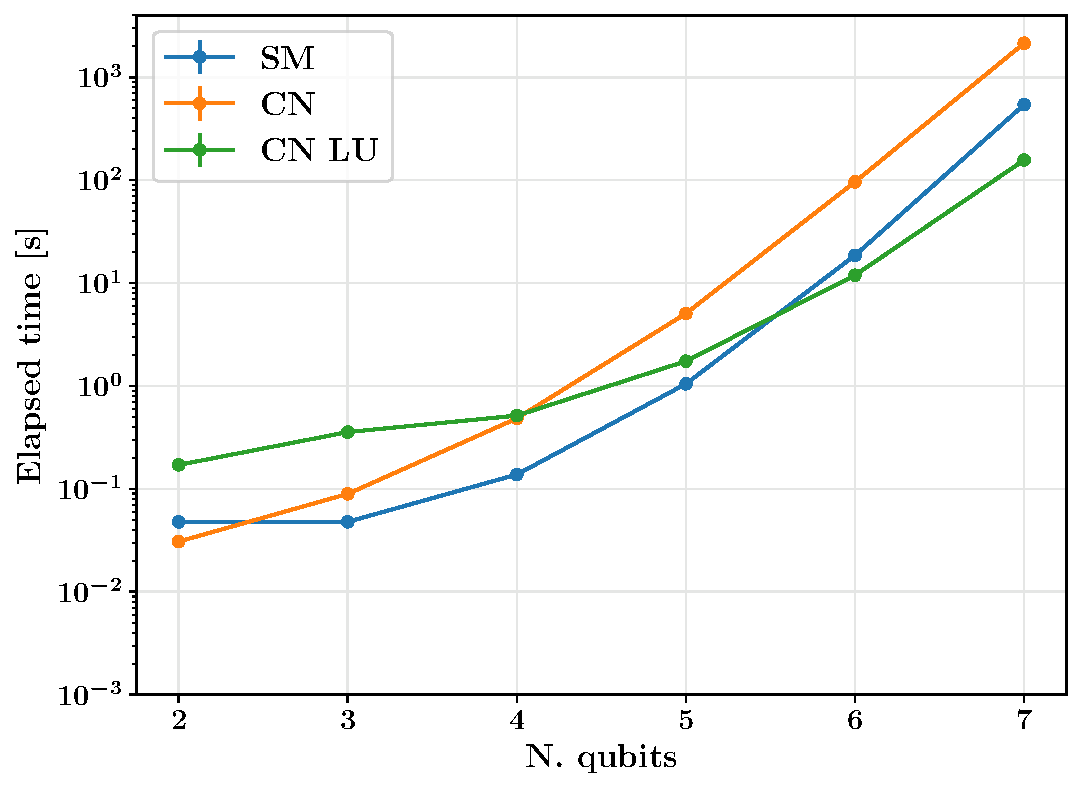
\includegraphics[width=1.0\textwidth]{image/timing/time_tensorflow_CPU.pdf} \label{fig:tensor_CPU} }
\end{minipage}
\begin{minipage}[]{0.49\linewidth}
\centering
\subfloat[][TensorFlow GPU]{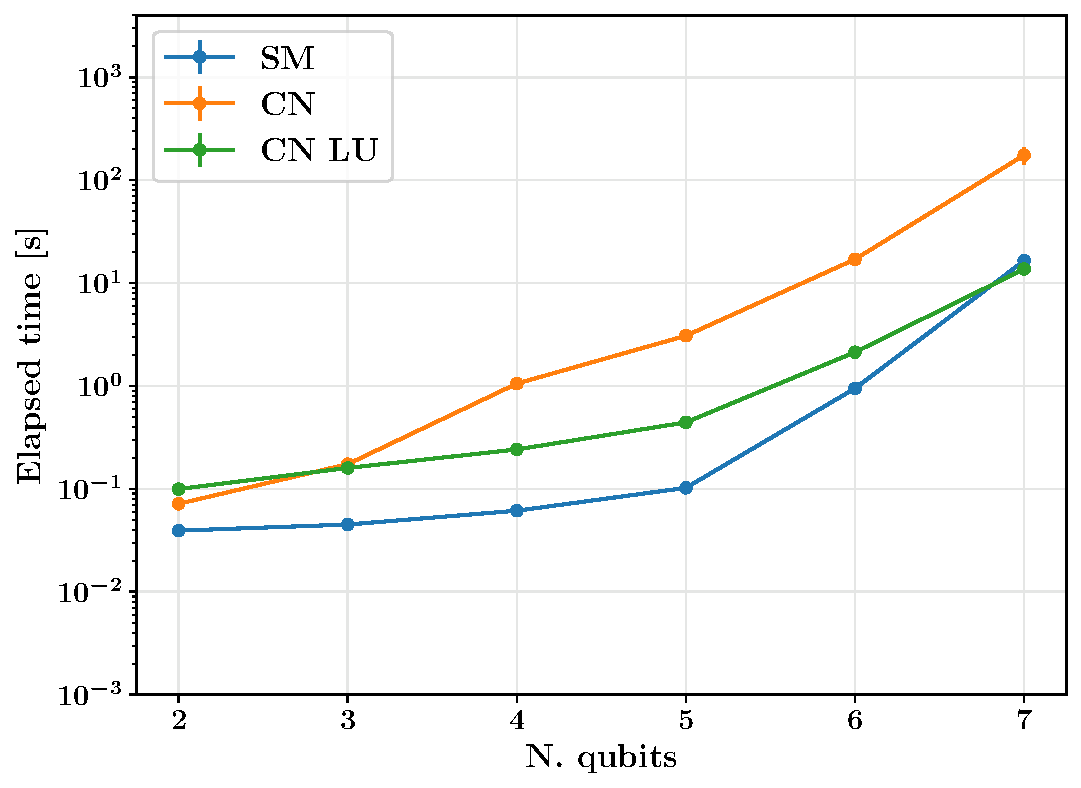
\includegraphics[width=1.0\textwidth]{image/timing/time_tensorflow_GPU.pdf}  \label{fig:tensor_GPU} }
\end{minipage}
\begin{minipage}[c]{0.49\linewidth}
\subfloat[][NumPy]{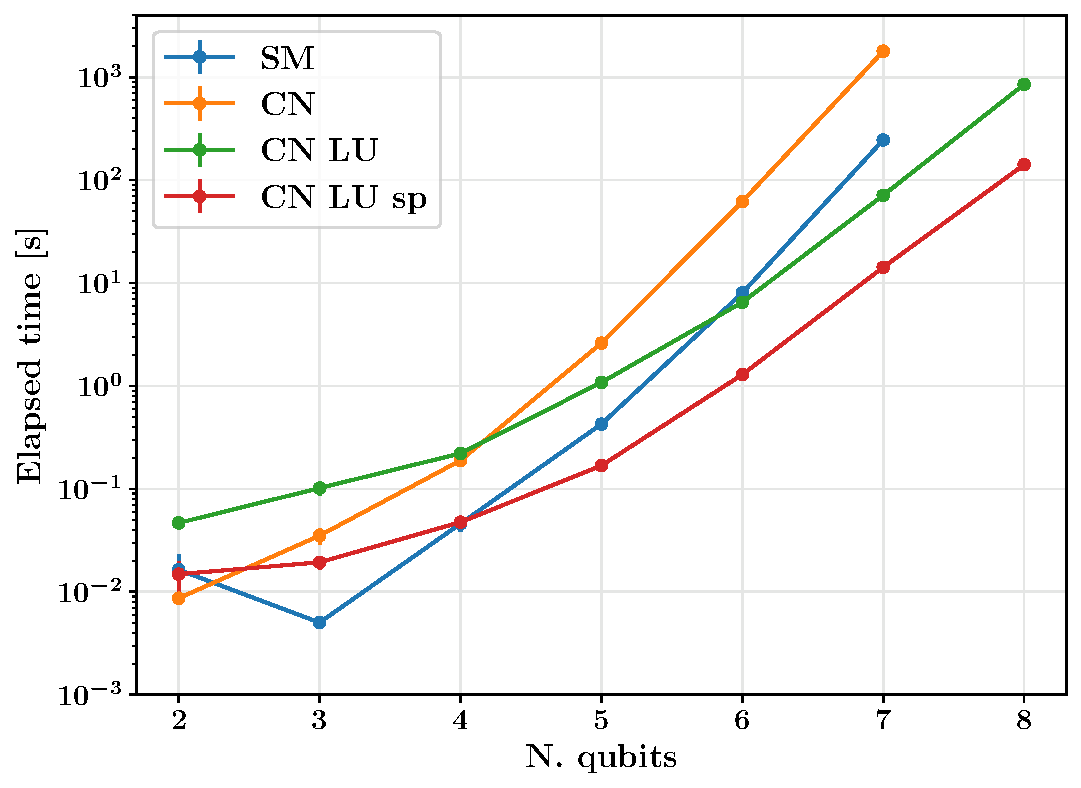
\includegraphics[width=1.0\textwidth]{image/timing/time_numpy.pdf} \label{fig:numpy} }
\end{minipage}
\begin{minipage}[c]{0.49\linewidth}
\subfloat[][Spectral Method Comparison]{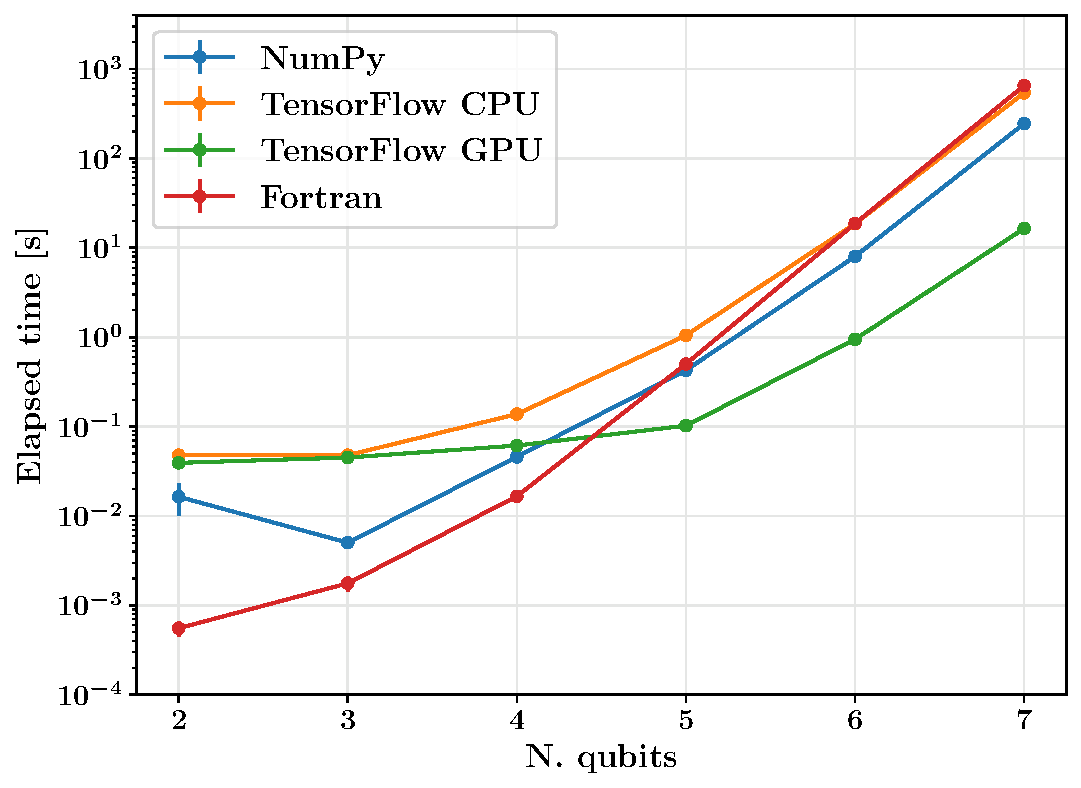
\includegraphics[width=1.0\textwidth]{image/timing/timing_spectral_comparison.pdf} \label{fig:comparison} }
\end{minipage}
\caption{Mean elapsed time in seconds as a function of the number of qubits in the chain. Spectral Method (SM), Crank-Nicolson method (CN),  Crank-Nicolson with LU decomposition method (CN LU) and Crank-Nicolson with LU decomposition with sparse matrix method (CN LU sp) are compared. We consider TensorFlow implementation on CPU (\ref{fig:tensor_CPU}),  TensorFlow implementation on GPU (\ref{fig:tensor_GPU}) NumPy implementation (\ref{fig:numpy}) and a comparison between all implementations with Spectral methods (\ref{fig:comparison}).}
\label{fig:timing}
\end{figure}

\clearpage

\section{Conclusions}
\label{sec:conclusions}

In this Report, we simulate numerically the dynamics of a two-qubit system under the application of a controlled-phase gate. 

First of all, we check the correctness of the numerical implementation by fixing the optimal parameters suggested and comparing the results with the one of \cite{PhysRevLett.123.170503}. 

Then, we vary the optimal parameters in order to investigate the behavior of the CZ gate in response to this variation. We see that a proper choice of $\Omega\tau$ and $\Delta/\Omega$ is needed so that a state initially in $\ket{11}$ return to itself after the CZ gate application. Instead, if the system is in $\ket{01}$ (or $\ket{10}$), it return to itself independently on the optimal choice of the parameters $\Omega\tau$ and $\Delta/\Omega$, but a proper choice of the phase jump between the two pulses is needed. The dynamical phase acquired both by $\ket{11}$ and $\ket{01}$ (or $\ket{10}$) depends strongly on this choice. This is a crucial point for a correct realization of a controlled-phase gate for which $\phi_{11}=2\phi_{01}-\pi$.

Moreover, a Gaussian noise is also introduced in the system and the measurement process is simulated, both in perfect and imperfect blockade regime, obtaining the expected results. In the last case, we note that increasing the strength parameter $V$, the state $\ket{rr}$ less and less likely.

After that, the CZ gate is implemented in a chain of $N$-qubit and also in this case a Gaussian noise before each pulse is provided. We perturb separately the parameter $\Omega\tau$ and $\Delta/\Omega$ and we monitor respectively the error $\epsilon$ and the relation $\phi_{11}=2\phi_{01}-\pi$.
In both cases, we do not observe any significant difference as a function of the standard deviation of the normal noise for different number of qubits.

Finally, a timing analysis of unitary time evolution algorithms and of their different implementations is performed. We conclude that for a lower number of qubits the spectral method have good performances especially in the TensorFlow GPU implementation. However, this method is not feasible for a larger number of qubits. Indeed, approximation are needed in order to handle such big matrices. One can rely on Crank-Nicolson algorithm with LU decomposition which for large matrices seems to scale slowly. Even better, it is the NumPy implementation of Crank-Nicolson algorithm with LU decomposition with sparse matrices.

All the implemented code and the results shown in this work are available on GitHub \cite{github}.

% To add bibliography (file references.bib)
\bibliographystyle{unsrt}
\bibliography{references}{}

\end{document}

